% Template LaTeX file for DAFx-20 papers
%
% To generate the correct references using BibTeX, run
%     latex, bibtex, latex, latex
% modified...
% - from DAFx-00 to DAFx-02 by Florian Keiler, 2002-07-08
% - from DAFx-03 to DAFx-04 by Gianpaolo Evangelista, 2004-02-07 
% - from DAFx-05 to DAFx-06 by Vincent Verfaille, 2006-02-05
% - from DAFx-06 to DAFx-07 by Vincent Verfaille, 2007-01-05
%                          and Sylvain Marchand, 2007-01-31
% - from DAFx-07 to DAFx-08 by Henri Penttinen, 2007-12-12
%                          and Jyri Pakarinen 2008-01-28
% - from DAFx-08 to DAFx-09 by Giorgio Prandi, Fabio Antonacci 2008-10-03
% - from DAFx-09 to DAFx-10 by Hannes Pomberger 2010-02-01
% - from DAFx-10 to DAFx-12 by Jez Wells 2011
% - from DAFx-12 to DAFx-14 by Sascha Disch 2013
% - from DAFx-15 to DAFx-16 by Pavel Rajmic 2015
% - from DAFx-16 to DAFx-17 by Brian Hamilton 2016
% - from DAFx-17 to DAFx-18 by Annibal Ferreira and Matthew Davies 2017
% - from DAFx-18 to DAFx-19 by Dave Moffat 2019
% - from DAFx-19 to DAFx-20 by Gianpaolo Evangelista 2019
%
% Template with hyper-references (links) active after conversion to pdf
% (with the distiller) or if compiled with pdflatex.
%
% 20060205: added package 'hypcap' to correct hyperlinks to figures and tables
%                      use of \papertitle and \paperauthorA, etc for same title in PDF and Metadata
% 20190205: Package 'hypcap' removed, and replaced with 'caption', to allow for the inclusion
%			of a CC UP licence.
%
% 1) Please compile using latex or pdflatex.
% 2) If using pdflatex, you need your figures in a file format other than eps! e.g. png or jpg is working
% 3) Please use "paperftitle" and "pdfauthor" definitions below

%------------------------------------------------------------------------------------------
%  !  !  !  !  !  !  !  !  !  !  !  ! user defined variables  !  !  !  !  !  !  !  !  !  !  !  !  !  !
% Please use the following commands to define title and author(s) of the paper.
% paperauthorA MUST be the the first author of the paper
% Please comment the unused definitions 
\def\papertitle{Dynamic Grids for Finite-Difference Schemes in Musical Instrument Simulations}
\def\paperauthorA{Silvin Willemsen}
\def\paperauthorB{Stefan Bilbao}
\def\paperauthorC{Michele Ducceschi}
\def\paperauthorD{Stefania Serafin}
%\def\paperauthorE{Author Five}
%\def\paperauthorF{Author Six}
%\def\paperauthorG{Author Seven}
%\def\paperauthorH{Author Eight}
%\def\paperauthorI{Author Nine}
%\def\paperauthorJ{Author Ten}

% Authors' affiliations have to be set below

%------------------------------------------------------------------------------------------
\documentclass[twoside,a4paper, dvipsnames]{article}
\usepackage{etoolbox}
\usepackage{dafx_20}
\usepackage{amsmath,amssymb,amsfonts,amsthm}
\usepackage{euscript}
%\usepackage[latin1]{inputenc}
\usepackage[T1]{fontenc}
\usepackage[utf8]{inputenc}
%\usepackage[T1]{fontenc}
%\usepackage{lmodern}
\usepackage{nimbusserif}
\usepackage{ifpdf}
\usepackage[english]{babel}
\usepackage{caption}
\usepackage{subfig} % or can use subcaption package
% \usepackage{color}
\usepackage{xcolor}
\makeatletter
\renewcommand*\env@matrix[1][*\c@MaxMatrixCols c]{%
  \hskip -\arraycolsep
  \let\@ifnextchar\new@ifnextchar
  \array{#1}}
\makeatother

\def\SBcomment[#1]{\textcolor{Red}{#1}}
\def\SWcomment[#1]{\textcolor{Cyan}{#1}}
\def\MDcomment[#1]{\textcolor{Green}{#1}}
\def\SScomment[#1]{\textcolor{Bittersweet}{#1}}
\DeclareMathAlphabet\mathbfcal{OMS}{cmsy}{b}{n}

\def\flip{\leftarrow}
\def\U{\mathbfcal{U}}
\def\Nfrac{\mathcal{N}}
\def\lu{{l_u}}
\def\lw{{l_w}}
\def\ugen{q} % general state variable to be used in the regular case (sections 2 and 3) 

\usepackage{cases}
% \usepackage{subfig}
\usepackage{algorithm2e, setspace}

\input glyphtounicode
\pdfgentounicode=1

\setcounter{page}{1}
\ninept

% build the list of authors and set the flag \multipleauth to handle the et al. in the copyright note (in DAFx_20.sty)
%==============================DO NOT MODIFY =======================================
\newcounter{numauth}\setcounter{numauth}{1}
\newcounter{listcnt}\setcounter{listcnt}{1}
\newcommand\authcnt[1]{\ifdefined#1 \stepcounter{numauth} \fi}

\newcommand\addauth[1]{
\ifdefined#1 
\stepcounter{listcnt}
\ifnum \value{listcnt}<\value{numauth}
\appto\authorslist{, #1}
\else
\appto\authorslist{~and~#1}
\fi
\fi}
%======DO NOT MODIFY UNLESS YOUR PAPER HAS MORE THAN 10 AUTHORS========================
%==we count the authors defined at the beginning of the file (paperauthorA is mandatory and already accounted for)
\authcnt{\paperauthorB}
\authcnt{\paperauthorC}
\authcnt{\paperauthorD}
\authcnt{\paperauthorE}
\authcnt{\paperauthorF}
\authcnt{\paperauthorG}
\authcnt{\paperauthorH}
\authcnt{\paperauthorI}
\authcnt{\paperauthorJ}
%==we create a list of authors for pdf tagging, for example: paperauthorA, paperauthorB, ... and paperauthorF (last author)
\def\authorslist{\paperauthorA}
\addauth{\paperauthorB}
\addauth{\paperauthorC}
\addauth{\paperauthorD}
\addauth{\paperauthorE}
\addauth{\paperauthorF}
\addauth{\paperauthorG}
\addauth{\paperauthorH}
\addauth{\paperauthorI}
\addauth{\paperauthorJ}
%====================================================================================

\usepackage{times}
% Saves a lot of ouptut space in PDF... after conversion with the distiller
% Delete if you cannot get PS fonts working on your system.


% pdf-tex settings: detect automatically if run by latex or pdflatex
\newif\ifpdf
\ifx\pdfoutput\relax
\else
   \ifcase\pdfoutput
      \pdffalse
   \else
      \pdftrue
\fi

\ifpdf % compiling with pdflatex
  \usepackage[pdftex,
    pdftitle={\papertitle},
    pdfauthor={\authorslist},
    pdfsubject={Proceedings of the 23rd International Conference on Digital Audio Effects (DAFx-20)},
    colorlinks=false, % links are activated as color boxes instead of color text
    bookmarksnumbered, % use section numbers with bookmarks
    pdfstartview=XYZ % start with zoom=100% instead of full screen; especially useful if working with a big screen :-)
  ]{hyperref}
  \pdfcompresslevel=9
  \usepackage[pdftex]{graphicx}
 % \usepackage[figure,table]{hypcap}
\else % compiling with latex
  \usepackage[dvips]{epsfig,graphicx}
  \usepackage[dvips,
    pdftitle={\papertitle},
    pdfauthor={\authorslist},
    pdfsubject={Proceedings of the 23rd International Conference on Digital Audio Effects (DAFx-20)},
    colorlinks=false, % no color links
    bookmarksnumbered, % use section numbers with bookmarks
    pdfstartview=XYZ % start with zoom=100% instead of full screen
  ]{hyperref}
  % hyperrefs are active in the pdf file after conversion
  %\usepackage[figure,table]{hypcap}
\fi
\usepackage[hypcap=true]{caption}
\title{\papertitle}

%-------------SINGLE-AFFILIATION SINGLE-AUTHOR HEADER STARTS (uncomment below if your paper has a single author)----------------------------------------
%\affiliation{
%\paperauthorA\,\sthanks{Thanks to the predecessors for the templates}}
%{\href{https://www.mdw.ac.at/ike/}{Institute 1} \\ University of Music and Performing Arts\\ Vienna, Austria\\
%{\tt \href{mailto:dafx2020@gmail.com}{dafx2020@gmail.com}}
%}
%
%Please note that the copyright notice should be separated from the text by a line (like a footnote). This works automatically when you have an \sthanks command 
%in the authors' line. However, if your paper does not require an \sthanks command, please use an empty (vertical space eating) \thanks command as follows:
%\affiliation{
%\paperauthorA\,\thanks{\vspace{-3mm}}}
%{\href{https://www.mdw.ac.at/ike/}{Institute 1} \\ University of Music and Performing Arts\\ Vienna, Austria\\
%{\tt \href{mailto:dafx2020@gmail.com}{dafx2020@gmail.com}}
%}
%-------------SINGLE-AFFILIATION SINGLE-AUTHOR HEADER ENDS-------------------------------------------------------------------------------------------------------------------

%------------SINGLE-AFFILIATION MULTIPLE-AUTHORS HEADER STARTS (uncomment below if your paper has two or more authors from the same institution)
%\affiliation{
%\paperauthorA\,\sthanks{Thanks to the predecessors for the templates}and \paperauthorB \,\sthanks{This work was supported by the XYZ Foundation}}
%{\href{https://www.mdw.ac.at/ike/}{Institute 1} \\ University of Music and Performing Arts\\ Vienna, Austria\\
%{\tt \href{mailto:dafx2020@gmail.com}{dafx2020@gmail.com}}
%}
%
%Please note that the copyright notice should be separated from the text by a line (like a footnote). This works automatically when you have an \sthanks command 
%in the authors' line. However, if your paper does not require an \sthanks command, please use an empty (vertical space eating) \thanks command as follows:
%\affiliation{
%\paperauthorA\ and \paperauthorB\,\thanks{\vspace{-3mm}}}
%{\href{https://www.mdw.ac.at/ike/}{Institute 1} \\ University of Music and Performing Arts\\ Vienna, Austria\\
%{\tt \href{mailto:dafx2020@gmail.com}{dafx2020@gmail.com} | \href{mailto:dafx2021@gmail.com}{dafx2020@gmail.com} }
%}
%-----------------------------------SINGLE-AFFILIATION-MULTIPLE-AUTHORS HEADER ENDS----------------------------------------------------------------------------------------

%---------------TWO-AFFILIATIONS HEADER STARTS (uncomment below if your paper has two authors, each from a different institution)-----------------------------
%\twoaffiliations{
%\paperauthorA \,\sthanks{Thanks to the predecessors for the templates}}
%{\href{https://www.mdw.ac.at/ike/}{Institute 1} \\ University of Music and Performing Arts\\ Vienna, Austria\\
%{\tt \href{mailto:dafx2020@gmail.com}{dafx2020@gmail.com}}
%}
%{\paperauthorB \,\sthanks{This work was supported by the XYZ Foundation}}
%{\href{http://dafx2019.bcu.ac.uk/}{Digital Media Technology Lab} \\ Birmingham City University \\ Birmingham, UK \\ {\tt \href{mailto:dafx2019@gmail.com}{dafx2019@gmail.com}}
%}
%
%Please note that the copyright notice should be separated from the text by a line (like a footnote). This works automatically when you have an \sthanks command 
%in the authors' line. However, if your paper does not require any \sthanks command, please use an empty (vertical space eating) \thanks command only in one of the authors
%headers as follows:
%\twoaffiliations{
%\paperauthorA \,\thanks{\vspace{-3mm}}}
%{\href{https://www.mdw.ac.at/ike/}{Institute 1} \\ University of Music and Performing Arts\\ Vienna, Austria\\
%{\tt \href{mailto:dafx2020@gmail.com}{dafx2020@gmail.com}}
%}
%{\paperauthorB \,}
%{\href{http://dafx2019.bcu.ac.uk/}{Digital Media Technology Lab} \\ Birmingham City University \\ Birmingham, UK \\ {\tt \href{mailto:dafx2019@gmail.com}{dafx2019@gmail.com}}
%}
%-------------------------------------TWO-AFFILIATIONS HEADER ENDS------------------------------------------------------

%%---------------THREE-AFFILIATIONS HEADER STARTS (uncomment below if your paper has three authors, each from a different institution)-----------------------
%\threeaffiliations{
%\paperauthorA \,\sthanks{Thanks to the predecessors for the templates}}
%{\href{https://www.mdw.ac.at/ike/}{Institute 1} \\ University of Music and Performing Arts\\ Vienna, Austria\\
%{\tt \href{mailto:dafx2020@gmail.com}{dafx2020@gmail.com}}
%}
%{\paperauthorB \,\sthanks{This work was supported by the XYZ Foundation}}
%{\href{http://dafx2019.bcu.ac.uk/}{Digital Media Technology Lab} \\ Birmingham City University \\ Birmingham, UK \\ {\tt \href{mailto:dafx2019@gmail.com}{dafx2019@gmail.com}}
%}
%{\paperauthorC \,\sthanks{Illustrious contributor}}
%{\href{http://dafx2018.web.ua.pt/}{IEETA} \\ University of Aveiro \\ Aveiro, Portugal \\ {\tt \href{mailto:dafx2018_papers@ua.pt}{dafx2018\_papers@ua.pt}}
%}
%
%Please note that the copyright notice should be separated from the text by a line (like a footnote). This works automatically when you have an \sthanks command 
%in the authors' line. However, if your paper does not require any \sthanks command, please use an empty (vertical space eating) \thanks command only in one of the authors
%headers as follows:
\threeaffiliations{
\paperauthorA \,}{{Multisensory Experience Lab} \\ Aalborg University Copenhagen\\ Copenhagen, Denmark\\
{\tt \href{mailto:sil@create.aau.dk}{sil@create.aau.dk}}
}
{\paperauthorB, \paperauthorC\,}
{{Acoustics and Audio Group} \\ University of Edinburgh \\ Edinburgh, UK
}
{\paperauthorD \,}
{{Multisensory Experience Lab} \\ Aalborg University Copenhagen\\ Copenhagen, Denmark}
%-------------------------------------THREE-AFFILIATIONS HEADER ENDS------------------------------------------------------

%----------------FOUR-AFFILIATIONS HEADER STARTS (uncomment below if your paper has four authors, , each from a different institution)-----------------------
% \fouraffiliations{
% \paperauthorA \,\sthanks{Thanks to the predecessors for the templates}}
% {\href{https://www.mdw.ac.at/ike/}{Institute 1} \\ University of Music and Performing Arts\\ Vienna, Austria\\
% {\tt \href{mailto:dafx2020@gmail.com}{dafx2020@gmail.com}}
% }
% {\paperauthorB \,\sthanks{This work was supported by the XYZ Foundation}}
% {\href{http://dafx2019.bcu.ac.uk/}{Digital Media Technology Lab} \\ Birmingham City University \\ Birmingham, UK \\ {\tt \href{mailto:dafx2019@gmail.com}{dafx2019@gmail.com}}
% }
% {\paperauthorC \,\sthanks{Illustrious contributor}}
% {\href{http://dafx2018.web.ua.pt/}{IEETA} \\ University of Aveiro \\ Aveiro, Portugal \\ {\tt \href{mailto:dafx2018_papers@ua.pt}{dafx2018\_papers@ua.pt}}
% }
% {\paperauthorD \,\sthanks{This guy is a very good fellow}}
% {\href{http://www.acoustics.ed.ac.uk}{Acoustics and Audio Group} \\ University of Edinburgh\\ Edinburgh, UK\\ {\tt \href{mailto:dafx17@ed.ac.uk}{dafx17@ed.ac.uk}}
% }
%
%Please note that the copyright notice should be separated from the text by a line (like a footnote). This works automatically when you have an \sthanks command 
%in the authors' line. However, if your paper does not require any \sthanks command, please use an empty (vertical space eating) \thanks command only in one of the authors
%headers as follows:
%\fouraffiliations{
%\paperauthorA \,\thanks{\vspace{-3mm}}}
%{\href{https://www.mdw.ac.at/ike/}{Institute 1} \\ University of Music and Performing Arts\\ Vienna, Austria\\
%{\tt \href{mailto:dafx2020@gmail.com}{dafx2020@gmail.com}}
%}
%{\paperauthorB \,}
%{\href{http://dafx2019.bcu.ac.uk/}{Digital Media Technology Lab} \\ Birmingham City University \\ Birmingham, UK \\ {\tt \href{mailto:dafx2019@gmail.com}{dafx2019@gmail.com}}
%}
%{\paperauthorC \,}
%{\href{http://dafx2018.web.ua.pt/}{IEETA} \\ University of Aveiro \\ Aveiro, Portugal \\ {\tt \href{mailto:dafx2018_papers@ua.pt}{dafx2018\_papers@ua.pt}}
%}
%{\paperauthorD \,}
%{\href{http://www.acoustics.ed.ac.uk}{Acoustics and Audio Group} \\ University of Edinburgh\\ Edinburgh, UK\\ {\tt \href{mailto:dafx17@ed.ac.uk}{dafx17@ed.ac.uk}}
%}
%-------------------------------------FOUR-AFFILIATIONS HEADER ENDS------------------------------------------------------

\begin{document}
% more pdf-tex settings:
\ifpdf % used graphic file format for pdflatex
  \DeclareGraphicsExtensions{.png,.jpg,.pdf, .eps}
\else  % used graphic file format for latex
  \DeclareGraphicsExtensions{.eps}
\fi

%\makeatletter
%\pdfbookmark[0]{\@pdftitle}{title}
%\makeatother

\maketitle

\begin{abstract}
For physical modelling sound synthesis, many techniques are available; time-stepping methods (e.g., finite-difference time-domain (FDTD) methods) have an advantage of flexibility and generality in terms of the type of systems they can model. These methods do, however, lack the capability of easily handling smooth parameter changes 
while retaining optimal simulation quality and stability, something other techniques are better suited for. In this paper, we propose an efficient method to smoothly add and remove grid points from a FDTD simulation under sub-audio rate parameter variations. This allows for dynamic parameter changes in physical models of musical instruments. An instrument such as the trombone can now be modelled using FDTD methods, as well as physically impossible instruments where parameters such as e.g. material density or its geometry can be made time-varying. Results show that the method does not produce (visible) artifacts and stability analysis is ongoing.

% An instrument such as the trombone can now be modelled using FDTD methods, as well as physically impossible instruments. %Furthermore, this technique allows the stability condition that the schemes using FDTD methods are based on, to always be satisfied with equality and thus have the highest simulation quality possible.\SBcomment[Too technical for the abstract: can say "Stability analysis follows directly as in the static case"] \SWcomment[Does it? I haven't tried to perform stability analysis on the method yet..]\SBcomment[I don't know!] 

\end{abstract}
% \section{Introduction}

\SWcomment[something before this] Any musical instrument can be subdivided into an exciter and a resonator component \cite{Borin1989}. Examples of exciter-resonator combinations are the bow and violin and the lips and trumpet. In nearly all instruments, the variables describing the exciter are `modified' to play the instrument, i.e, the bow-velocity, position and pressure for the violin, and lip pressure and frequency for the trumpet. Naturally, the resonator is altered by fingering the strings of the violin or pressing valves on the trumpet to change its pitch. The variables describing the physics of the resonator itself are not changed though; the string-length stays the same and the total tube length remains unchanged, only the parts that resonate are shortened or lengthened.

In some cases, though, the parameters describing the resonator are modified. A prime example of this is the trombone, where the tube length is dynamically changed in order to generate different pitches. The slide whistle is another example in this category. Guitar strings are another category where the tension can be smoothly modulated during performance using the fretting finger, a whammy bar or even the tuning pegs directly (see \cite{Gomm2011}) to create smooth pitch glides. The same kind of tension modulation is used for the membranes of timpani or ``hourglass drums" to change the pitch. %or pressing down on the strings of a hammered dulcimer on one side of a bridge, while playing the string on the other side for the same effect \cite{Glenn2014}. 
It is these direct parameter modifications of the resonators that we are interested in to simulate.
%Among the reasons of why one would simulate an instrument rather than sample an existing one, is that one could extend the capabilities of this instrument beyond what is physically possible, such as changing material properties or size of the instrument dynamically.

% of simulating musical instruments rather than recording them and playing them back (samples), is the flexibility of control and playability of the instrument. Imagine trying to record the entire control space of a violin, i.e., all possible combinations of bowing force, bowing velocity and fingering positions. The recording procedure would take a great amount of time and resources, let alone the amount of data storage required to store all of the high-quality audio.

% Due to the vast parameter space of many instruments, using simulations is a much more viable solution for capturing the full expressivity of an instrument than sampling.
% Some instruments require their parameters to be changed in order to be played. The first instrument that comes to mind is the trombone, where the geometry of the system, i.e., the tube length, is dynamically varied to produce different pitches. 

Other than simulating existing instruments, one can simulate instruments that can be manipulated in physically impossible ways. %\SBcomment[OK, it's good to have this in here, but this is immediately kind of a red flag for JASA, where they'd expect you to be attacking a problem from the real world first. Otherwise, they might well say that this belongs in CMJ. So: suggesting referring to real world examples first, then bring up the idea of imaginary instruments... ] \SWcomment[Will do!] 
Examples of this could be to dynamically change material properties such as density or stiffness, or even the geometry and size of the instrument. %An example of a real-world instrument that requires these manipulations is the trombone, where tube length is dynamically controlled by the player.

% This can be extended from musical instruments to rooms and acoustic simulation with variable shapes

Simulating musical instruments using physical modelling is a well-established field. Existing physical modelling techniques that have shown their ability to implement dynamic parameter changes of resonators include digital waveguides (DWGs) \cite{Smith1992} and modal synthesis \cite{morrison1993mosaic}. Literature using DWGs for time-varying parameters include Michon's BladeAxe \cite{Michon2014,Michon2016} and Cook's ... \SWcomment[SOTA on trombone / variable parameters with waveguides here!]

Modal synthesis, though requiring some assumptions and simplifications for most systems, does allow for easy and smooth parameter changes. Resonant frequencies of the different modes can be dynamically modified without many issues as long as modal frequencies exceeding the stability condition are excluded as parameters are changed. Examples can be found in \cite{Willemsen2017} and \cite{Mehes2016, Mehes2017, Walstijn2017} \SWcomment[$\leftarrow$ maybe not all of these van Walstijn papers]. Modal synthesis could thus be a good candidate for implementing the aforementioned dynamic parameters. In the case of the trombone, however, due to its non-homogenous geometry, there is no closed-form solution available and the modes would need to be calculated for every single slide configuration.

Finite-difference time-domain (FDTD) methods on the other hand, though generally more computationally expensive than other techniques, are flexible and generalisable and do not need as many simplifications as modal synthesis does. %\SBcomment[OK, I think reviewers may not like this at all. Particularly in the case of the trombone, where people like Perry Cook were doing things with variable delay lines (I think) a long time ago. if a waveguide person gets this for review, they will probably get annoyed. ] 
FDTD methods subdivide continuous partial differential equations (PDEs) that describe the physics of the system at hand into a grid of discrete points in space and time. \SWcomment[slightly different wording here $\rightarrow$] The challenge when trying to implement systems with dynamic parameters using FDTD methods, is that the number of grid points used in the simulation is closely tied to the parameters themselves \SWcomment[through a stability condition]. Adding and removing points from the grid is nontrivial and could cause audible artefacts or instability of the simulation. Full-grid interpolation \cite[Ch. 5]{bilbao2009} could be a possible solution here, but extremely high sample rates are necessary to avoid audible artefacts and low-passing effects when changing between grid configurations. 

% Below, a brief introduction about grids and their relationship to stability is explained.
%
% \subsection{Grids and stability}
% The distance between two discrete points in space (known as grid spacing) and the time step between two discrete moments in time are closely connected through a \textit{stability condition}. This condition dictates the maximum number of points allowed to describe a system before it gets unstable and the simulation ``explodes''. The closer the grid spacing is to the stability condition, the higher the quality of the simulation. If the condition is satisfied with equality, the quality of the simulation is at a maximum. \SBcomment[OK, this whole argument above seems out of place at little. Plus there are no references, or an indication of what quality means. As in: reviewers probably will not grasp why this is an important problem to solve. I suggest removing. Better to focus attention here away from the detailed numerical details (like grid spacings and numerical stability conditions and stuff) as the reviewers will probably see these as just small technical details. The important thing is the dynamic behaviour...] \SWcomment[Yes, I completely agree, the introduction mainly consists of notes at this point, some that were left from when I started writing this paper long ago :)]
% Furthermore, the stability condition depends on the parameters of the model, such as material properties or size of the system, i.e., parameters that could be changed on the fly \SBcomment[As above].

This article proposes an efficient method to smoothly add and remove points from 1D finite-difference grids to allow for dynamic parameter changes. We are interested in `slowly' varying parameters (sub-audio rate) \SWcomment[so that modal and energetic analysis techniques are still meaningful to a degree]. One can consider this work an introduction to implementing the trombone using FDTD methods.

\SWcomment[Only if there is space $\rightarrow$] This paper is structured as follows:

\section{Introduction}
The operation of most musical instruments can be subdivided into excitation and resonator components \cite{Borin1989}. Examples of excitation-resonator combinations are the bow and violin and the lips and trumpet. In some instruments, the parameters describing the excitation are continuously varied by the performer to play the instrument. As an example, the bow velocity, bow position and bow force for stringed instruments, and lip pressure and frequency for brass instruments. Naturally, the resonator is also altered by fingering the strings of the violin or pressing valves on the trumpet to change the instrument pitch. But, even under such variable playing conditions, physical properties of the resonators do not change: the string length and tension stay the same and the total tube length remains unchanged; it is only the portions that resonate that are shortened or lengthened.

There are several examples where the parameters of the resonator are also modified. A prime example of this is the trombone, where the tube length is dynamically changed in order to generate different pitches. The slide whistle is another example in this category. Guitar strings are another category where the tension can be smoothly modulated during performance using the fretting finger or a whammy bar  %or even the tuning pegs directly (see \cite{Gomm2011}) 
to create smooth pitch glides. The same kind of tension modulation is used for the membranes of timpani or ``hourglass drums" to change the pitch. 
It is these direct parameter modifications of the resonators that we are interested in simulating. In addition to simulating existing instruments, one could potentially simulate instruments that can be manipulated in physically impossible ways. Examples of this could be to dynamically change material properties such as density or stiffness, or even the geometry and size of the instrument where this is physically impossible.

Finite-difference time-domain (FDTD) methods are flexible and generalisable techniques which have seen increased use in physical modelling sound synthesis applications \cite{bilbao2009}. The normal approach, for a given system such as a musical instrument, is to describe its motion by a set of partial differential equations (PDEs). The instrument is then represented over a spatio-temporal grid, yielding a fully discrete approximation to the target PDE system. 

In many cases, the system itself is static, so that the defining parameters do not change over time. In others, such as the trombone and others mentioned above, this is not the case, and various technical challenges arise when trying to design a simulation using FDTD methods; all relate to the choice of the spatial grid. For example, the grid density is usually closely tied to the parameters themselves through a stability condition.
Also, adding and removing points from the grid is nontrivial and can cause audible artifacts and new stability concerns. The default approach of defining a grid globally, according to a very conservative stability condition, as done in \cite{Willemsen2019}, is possible, but introduces numerical dispersion and bandlimiting effects. Full-grid interpolation \cite[Ch. 5]{bilbao2009} could be used to change between grid configurations, but extremely high sample rates are necessary to avoid audible artifacts and low-passing effects, rendering any implementation offline. 

In this paper, a new method is proposed, allowing the efficient and smooth insertion and deletion of grid points from 1D finite-difference grids to allow for dynamic parameter changes. We are interested in varying parameters `slowly' (i.e., at sub-audio rate corresponding to human gestural control). In a companion paper we present a physical model of the trombone using the method proposed in this paper \cite{Willemsen2021}. Notice that other techniques do allow for dynamic parameter changes but come with their own drawbacks \cite{bilbao2009}. Examples of dynamic parameters using modal synthesis \cite{morrison1993mosaic} are shown in \cite{Mehes2016, Willemsen2017} and digital waveguides \cite{Smith1992} in \cite{Michon2014}.

%Among the reasons of why one would simulate an instrument rather than sample an existing one, is that one could extend the capabilities of this instrument beyond what is physically possible, such as changing material properties or size of the instrument dynamically.

% of simulating musical instruments rather than recording them and playing them back (samples), is the flexibility of control and playability of the instrument. Imagine trying to record the entire control space of a violin, i.e., all possible combinations of bowing force, bowing velocity and fingering positions. The recording procedure would take a great amount of time and resources, let alone the amount of data storage required to store all of the high-quality audio.

% Due to the vast parameter space of many instruments, using simulations is a much more viable solution for capturing the full expressivity of an instrument than sampling.
% Some instruments require their parameters to be changed in order to be played. The first instrument that comes to mind is the trombone, where the geometry of the system, i.e., the tube length, is dynamically varied to produce different pitches. 

 %\SBcomment[OK, it's good to have this in here, but this is immediately kind of a red flag for JASA, where they'd expect you to be attacking a problem from the real world first. Otherwise, they might well say that this belongs in CMJ. So: suggesting referring to real world examples first, then bring up the idea of imaginary instruments... ] \SWcomment[Will do!] 
 %An example of a real-world instrument that requires these manipulations is the trombone, where tube length is dynamically controlled by the player.

% This can be extended from musical instruments to rooms and acoustic simulation with variable shapes
% \SBcomment[OK, here, need that boring paragraph saying what's in each section in the paper...] \SWcomment[Haha, yeah thought so... Was hoping to exclude it for space...]

This paper is structured as follows: Section \ref{sec:continuous} presents the 1D wave equation, to be used as an illustrative example for the proposed method. Section \ref{sec:FDTD} gives an introduction to numerical methods, stability and simulation quality. The proposed method for dynamic grids is then presented in Section \ref{sec:dynamicGrid} and applied to the 1D wave equation. Section \ref{sec:results} shows the results of an analysis performed on the method, which are discussed in Section \ref{sec:discussion}. Finally, concluding remarks and future perspectives are given in \ref{sec:conclusion}.
\section{Continuous Systems}\label{sec:continuous}
%
%going from a partial differential equation (PDE) to an update equation that can be implemented.
%
%using the famous 1D wave equation.
%
The physics of dynamic systems is commonly described using partial differential equations (PDEs) operating in continuous time. To aid the illustration of the proposed method, the 1D wave equation will be used. This does not mean that the method is limited to this, and could be extended to other systems, possibly even higher dimensional ones.

The 1D wave equation may be written
\begin{equation}\label{eq:1dwave}
    \frac{\partial^2 u}{\partial t^2}= c^2\frac{\partial^2 u}{\partial x^2}\ ,
\end{equation}
and is defined over spatial domain $x \in [0, L]$, for length $L$ (in m) and time $t \geq 0$ (in s). $c$ (in m/s) is the wave speed. The dependent variable $u(x,t)$ in Eq. \eqref{eq:1dwave} may be interpreted as the transverse displacement of an ideal string, or the acoustic pressure in the case of a cylindrical tube. Two possible choices of boundary conditions are
\begin{subequations}\label{eq:continuousBoundaries}
    \begin{align}
        u(0, t) = u(L, t) &= 0\quad \text{(Dirichlet)},\label{eq:contDirichlet}\\
        \frac{\partial}{\partial x} u(0, t) = \frac{\partial}{\partial x} u(L, t) &= 0\quad \text{(Neumann)},\label{eq:contNeumann}
    \end{align}
\end{subequations}
which describe a `fixed' and `free' boundary respectively in the case of an ideal string, and `open' and `closed' conditions respectively in the case of a cylindrical acoustic tube.

\subsection{Dynamic parameters}\label{sec:dynamicParamsCont}
In the case of the 1D wave equation, only the wave speed $c$ and length $L$ can be altered. If Dirichlet-type boundary conditions -- as in Eq. \eqref{eq:contDirichlet} -- are used, and under static conditions the fundamental frequency $f_0$ of the 1D wave equation can be calculated according to
\begin{equation}\label{eq:fundamentalFreqCont}
    f_0 = \frac{c}{2L}.
\end{equation}
In the dynamic case, and under slow (sub-audiorate) variations of $c$ or $L$, Eq. \eqref{eq:fundamentalFreqCont} still approximately holds.
% \SBcomment[OK, but this notion of a frequency is only true under static conditions...kind of confusing] \SWcomment[Is it? It should be true for the dynamic case as well right?]\SBcomment[Well, I guess under slow variations, you can sort of say that there are still modes...but in general once you have time varying behaviour, you lose the ability to do Fourier analysis easily, and the modal analysis is not strictly correct] \SWcomment[Hmm.. but if this is true for any static combination of $c$ and $L$ (which it is right?) wouldn't it be true for the dynamic case as well?]\SBcomment[No way. It's approximately true for sub-audio rate variation in $c$. But once the variation gets higher, you will start to see AM effects (sidebands!).All modal analysis requires LTI behaviour. You can say that if the rate of variation of $c$ is sufficiently slow, then the modal frequencies above are approximately valid... ] \SWcomment[Ah of course, gotcha!]
%
From Eq. \eqref{eq:fundamentalFreqCont}, one can easily conclude that in terms of fundamental frequency, halving the length of Eq. \eqref{eq:1dwave} is identical to doubling the wave speed and vice versa. Looking at Eq. \eqref{eq:1dwave} in isolation, $f_0$ is the only behaviour that can be changed. One can thus leave $L$ fixed %($L = 1$ for simplicity) 
and make $c$ dynamic (or time-varying), i.e., $c = c(t)$, which will prove easier to work with in the following section.
\SBcomment[OK: here, need to refer back to the two primary cases here: the trombone, and the string under variable tensioning, and justify the use of a time-varying $c$ only in these cases. Otherwise this becomes too abstract. ] {\color{Cyan} I feel like I need to talk about scaling here and how this confirms this statement ($f_0 = \gamma/2$ with $\gamma = c/L$ and scaled space $x \in [0, 1]$).}
\section{Numerical methods}\label{sec:FDTD}
This section will provide a brief introduction to physical modelling using FDTD methods, including details on stability and quality of the simulations based on these methods. In the following, $c$ is assumed constant.

\subsection{Discretisation}
In FDTD methods, the first step is the definition of a grid. The spatial variable can be discretised using $x_l = lh$ %(read: $x$ at spatial index $l$) 
with integer $l \in \{0, \hdots, N\}$. The grid spacing $h$ (in m) is the distance between adjacent grid points, and the total number of points covering the domain, including endpoints, is $N + 1$. Here, integer $N$ describes the total number of intervals between the grid points, and thus the total domain length is $L=Nh$.
%is described as
% \begin{equation}\label{eq:numberOfIntervals}
%     N = \lfloor L/h\rfloor,
% \end{equation}
% \SBcomment[Easier to write this as $h=L/N$, for integer $N$, so without a flooring operation.] \SWcomment[hmm.. this flooring operation is important for the comparison with $\Nfrac$ (fractional $N$) later on. Just clearly shows $N$ ``integerness" :)]\SBcomment[OK, but from the above, we don't have $L=Nh$, so the total domain length is off...well, at least for a standard domain!]\SWcomment[gotcha, I'll figure this out.. (something with \eqref{eq:orderOfCalcGrid} perhaps..)]
%with $\lfloor \cdot \rfloor$ denoting the flooring operation. 
The temporal variable can be discretised using $t_n = nk$ with positive integer $n$, time step $k = 1/f_\text{s}$ (in s) for sample rate $f_\text{s}$ (in Hz). The state variable $\ugen$ can then be approximated using 
$q_{l}^{n}\approxeq q(x=lh,t=nk)$. 
% $\ugen(x,t) \approx \ugen_l^n$, where grid function $\ugen_l^n$ approximates $\ugen$ at spatial index $l$ and time index $n$. %The total state at time index $n$ is then denoted as vector $\mathbf{u}^n$ with size $N+1$.

The following operators can then be applied to $\ugen_l^n$ to get the following approximations to the derivatives in Eq. \eqref{eq:1dwave}
\begin{subequations}\label{eq:operators}
    \begin{align}
         \delta_{tt}\ugen_l^n &= \frac{1}{k^2}\left(\ugen_l^{n+1}-2\ugen_l^n + \ugen_l^{n-1}\right)\;\;\approx\quad\frac{\partial^2\ugen}{\partial t^2}\label{eq:secondOrderTime}\ ,\\
         \delta_{xx}\ugen_l^n &= \frac{1}{h^2}\left(\ugen_{l+1}^n-2\ugen_l^n + \ugen_{l-1}^n\right)\quad\approx\quad \frac{\partial^2\ugen}{\partial x^2}\ .\label{eq:secondOrderSpace}
    \end{align}
\end{subequations}
Substituting these definitions into Eq. \eqref{eq:1dwave} yields the following finite-difference scheme (FDS)
\begin{equation}\label{eq:FDS}
    \delta_{tt}\ugen_l^n = c^2 \delta_{xx}\ugen_l^n.
\end{equation}
%
Expanding the operators as in %the Eqs. in
\eqref{eq:operators} and solving for $\ugen_l^{n+1}$ yields the following update equation
\begin{equation}\label{eq:updateEq}
    \ugen_l^{n+1} = 2\ugen_l^n-\ugen_l^{n-1} + \lambda^2 \left(\ugen_{l+1}^n-2\ugen_l^n + \ugen_{l-1}^n\right).
\end{equation}
%saying that $\ugen$ at the next time index ($n+1$) can be calculated using only values of $\ugen$ at the current ($n$) and previous time indices ($n-1$).
which is suitable for direct software implementation. %This update can then be implemented in software, such as {\tt MATLAB} or {\tt C++}. 
Here,
\begin{equation}\label{eq:lambdaDef}
    \lambda = \frac{ck}{h}
\end{equation}
is referred to as the Courant number, constrained by numerical stability conditions, and also has an impact on the quality and behaviour of the simulation. This will be described in detail in Sections \ref{sec:stability} and \ref{sec:quality}.

In the FDS \SBcomment[Suggest chaging FDS globally to FDTD scheme or FD scheme, for consistency.]described in Eq. \eqref{eq:FDS}, the boundary locations are at $l = 0$ and $l = N$. Substituting these locations into Eq. \eqref{eq:updateEq} seemingly introduces the need of grid points outside of the defined domain, namely $\ugen_{-1}^n$ and $\ugen_{N+1}^n$. These can be referred to as \textit{virtual grid points} and can be accounted for using the boundary conditions in Eq. \eqref{eq:continuousBoundaries}. Discretising these yields
\begin{subequations}
    \begin{align}
        \ugen_0^n = \ugen_N^n &= 0 \quad\text{(Dirichlet)}\label{eq:discreteDirichlet}\\
        \delta_{x\cdot} \ugen_0^n = \delta_{x\cdot} \ugen_N^n &= 0 \quad \text{(Neumann)}\label{eq:discreteNeumann}
    \end{align}
\end{subequations}
where 
\begin{equation}
    \delta_{x\cdot}\ugen_l^n = \frac{1}{2h}\left(\ugen_{l+1}^n - \ugen_{l-1}^n\right)\quad \approx\quad \frac{\partial \ugen}{\partial x}
\end{equation}
is a second-order accurate approximation of the first-order spatial derivative. The Dirichlet condition in \eqref{eq:discreteDirichlet} says that the displacements of $\ugen$ at the boundary locations are always 0. In practice, this means that these grid points do not need to be updated and the spatial range of calculation for Eq. \eqref{eq:updateEq} then becomes $l \in \{1, \hdots, N-1\}$. If the Neumann condition is used, the boundary points do need to be updated as these are not necessarily $0$; rather, their `slope' is $0$. Eq. \eqref{eq:discreteNeumann} can then be expanded to yield defnitions for these virtual grid points
\begin{equation}\label{eq:neumannSolution}
    \ugen_{-1}^n = \ugen_1^n \quad \text{and} \quad \ugen_{N+1}^n = \ugen_{N-1}^n\,.
\end{equation}

Now that the full system is described, audio output at sample rate $f_\text{s}$ can be drawn from the state $\ugen_l^n$ in Eq. \eqref{eq:updateEq} at $0 < l < N$ (when using Dirichlet boundary conditions). %Though the output location does not change the behaviour of the system, it will determine the amplitude of different harmonic partials in the system output.

\subsection{Stability}\label{sec:stability}
Explicit FDTD methods for hyperbolic systems such as the 1D wave equation must necessarily satisfy a stability condition. In the case of the update in Eq. \eqref{eq:updateEq} it can be shown -- using von Neumann analysis \cite{Strikwerda1989} -- that the system is stable if
\begin{equation}\label{eq:CFL}
    \lambda \leq 1,
\end{equation}
which is referred to as the Courant-Friedrichs-Lewy (CFL) condition. The more closely $\lambda$ approaches this condition with equality, the higher the quality of the simulation (see Section \ref{sec:quality}) and if $\lambda = 1$, Eq. \eqref{eq:updateEq} yields an exact solution to Eq. \eqref{eq:1dwave}%(this is true for the 1D wave equation)
% (see Figures \ref{fig:dispersion}a and \ref{fig:dispersion}b)
. If $\lambda > 1$ the system will become unstable.
%  (see Figures \ref{fig:dispersion}a and \ref{fig:dispersion}b)
%
% \begin{figure}[t]
%     \centering
%     % \subfloat[]{\label{fig:lambda1}{ \includegraphics[width=0.3\textwidth]{Figures/ulnLambda1.eps}}}
%     % \subfloat[]{\label{fig:lambda0.9}{ \includegraphics[width=0.3\textwidth]{Figures/ulnLambda09.eps}}}
%     % \subfloat[]{\label{fig:lambda1.001}{ \includegraphics[width=0.3\textwidth]{Figures/ulnLambda1001.eps}}}
%     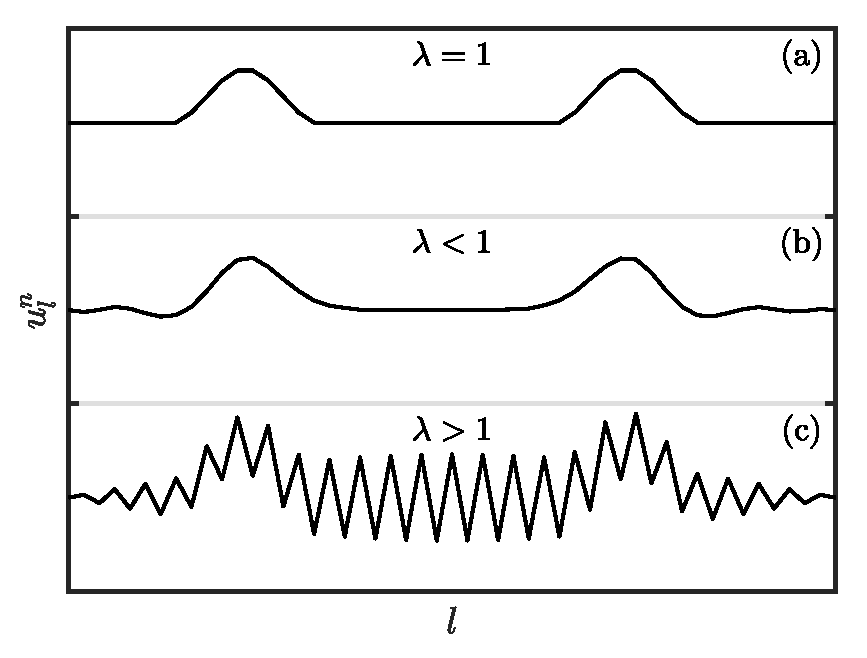
\includegraphics[width=0.8\columnwidth]{Figures/dispersionCompact.eps}
%     \caption{State $\ugen_l^n$ with $N = 50$ and $f_\text{s} = 44100$ visualised $\sim\!100$ samples after excitation. (a) If $\lambda = 1$, the solution is exact. (b) If $\lambda < 1$ dispersive behaviour shows. (c) If $\lambda > 1$ the CFL condition in Eq. \eqref{eq:CFL} is not satisfied and the system is unstable. \SWcomment[If $\ugen$ is used, don't forget to change in the figure!!]
%     \label{fig:dispersion}}
% \end{figure}
%
Recalling \eqref{eq:lambdaDef}, Eq. \eqref{eq:CFL} can be rewritten in terms of grid spacing $h$ to get
\begin{equation}\label{eq:stabilityCond}
    h \geq ck.
\end{equation}
This shows that the CFL condition in \eqref{eq:CFL} puts a lower bound on the grid spacing, determined by the sample rate and wave speed. Usually, the following steps are taken to calculate $\lambda$:
\begin{equation}\label{eq:orderOfCalcGrid}
    h := ck,\ \ N := \left\lfloor\frac{L}{h}\right\rfloor, \ \ h := \frac{L}{N}, \ \ \lambda := \frac{ck}{h}.
\end{equation}
In other words, condition \eqref{eq:stabilityCond} is first satisfied with equality and used to calculate number of intervals $N$. Thereafter, $h$ is recalculated based on integer $N$ and used to calculate $\lambda$. The calculation of $\lambda$ in Eq. \eqref{eq:orderOfCalcGrid} can be compactly rewritten as
\begin{equation}\label{eq:compactLambda}
    \lambda = \frac{ck}{L}\cdot\left\lfloor\frac{L}{ck}\right\rfloor.
\end{equation}
The flooring operation causes the CFL condition in \eqref{eq:CFL} to not always be satisfied with equality and results in a reduced simulation quality described in the following section.

\subsection{Simulation Quality}\label{sec:quality}
%As mentioned above, the Courant number $\lambda$ decides the quality of the simulation. 
Choosing $\lambda < 1$ in Eq. \eqref{eq:updateEq} will decrease the simulation quality in two ways. Firstly, it will decrease the maximum frequency that the simulation is able to produce, i.e., it will decrease the bandwidth of the output sound of the system. 
%See Figure \ref{fig:bandWidths}.

% \begin{figure}[t]
%     \centering
%     % \subfloat[]{\label{fig:bandwidth1}{ \includegraphics[width=0.3\textwidth]{Figures/bandwidthLambda1.eps}}}
%     % \subfloat[]{\label{fig:bandwidth09}{ \includegraphics[width=0.3\textwidth]{Figures/bandwidthLambda09.eps}}}
%     % \subfloat[]{\label{fig:bandwidth05}{ \includegraphics[width=0.3\textwidth]{Figures/bandwidthLambda05.eps}}}
%     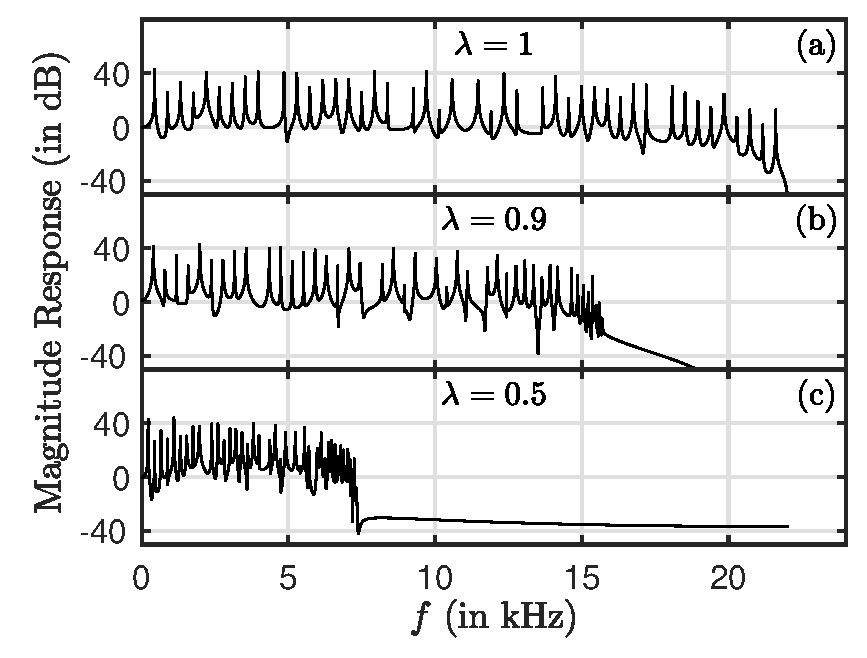
\includegraphics[width=0.9\columnwidth]{Figures/bandwidthCompact.eps}
%     \caption{Bandwidths of the simulation output %at $l = 16$ 
%     with $f_\text{s} = 44100$ Hz and 
%     %$N = 50$ excited with a raised cosine with a width of 5 at center-location $N = 25$. The Courant number is set to 
%     (a) $\lambda = 1$, (b) $\lambda = 0.9$ and (c) $\lambda = 0.5$. 
%     \label{fig:bandWidths}}
% \end{figure}
%
By analysing the scheme in Eq. \eqref{eq:updateEq}, it can be shown that the maximum frequency produced by the system can be calculated using $f_\text{max} = f_\text{s} \sin^{-1}(\lambda)/\pi$ \cite[Chap. 6]{bilbao2009}.
% \begin{equation}\label{eq:fmax}
%     f_\text{max} = \frac{f_\text{s}}{\pi} \sin^{-1}(\lambda).
% \end{equation}
% shown in Figure \ref{fig:bandWidthFormula}.
%
Note that only a small deviation of $\lambda$ from condition \eqref{eq:CFL} leads to a large reduction in output bandwidth.
%
% \begin{figure}
% %% \reprintcolumnwidth is the same in preprint and reprint for
% %% ease of use for authors:
% \includegraphics[width=0.8\reprintcolumnwidth]{bandwidthPlot}
% \caption{\label{fig:bandWidthFormula}{The effect of the Courant number $\lambda$ on the output bandwidth. \SWcomment[This figure should probably be much more compact, if not removed altogether.]}}
% \end{figure} 
Secondly, choosing $\lambda < 1$ causes numerical dispersion. %See Figures \ref{fig:dispersion}b and \ref{fig:bandWidths}. 
Harmonic partials become unnaturally closely spaced at higher frequencies (i.e. spurious inharmonicity increases) as $\lambda$ decreases, which is generally undesirable.

%\SWcomment[can cut this paragraph $\rightarrow$] Apart from the recalculation of $\lambda$ due to the flooring operation in Eq. \eqref{eq:orderOfCalcGrid}, a reason that one would choose $\lambda < 1$ could be to decrease the total number of grid points used in the simulation by increasing $h$. This makes the simulation less computationally expensive, while keeping a desired wave speed $c$ and time step $k$. For 1-dimensional systems such as the 1D wave equation, this is rarely necessary.

\section{Dynamic Parameters}\label{sec:dynamicParams}
This section describes how parameters could be made dynamic using FDTD methods using the state of the art. % and what this means for the simulation quality detailed in Section \ref{sec:quality}. %To clarify, for a parameter to be dynamic refers to its ability to vary over time while the simulation is running.  
To clarify, a \textit{dynamic} parameter refers to one that is time-varying while the simulation is running. 

% For the 1D wave equation used in Section \ref{sec:FDTD}, a property that could be interesting to make time-varying is the fundamental frequency $f_0$. If Dirichlet-type boundary conditions are used, as defined in Eqs. \eqref{eq:contDirichlet} and \eqref{eq:discreteDirichlet}, $f_0$ can be calculated according to
% \begin{equation}\label{eq:fundamentalFreq}
%     f_0 = \frac{c}{2L}\,.
% \end{equation}
% If $\lambda = 1$ in \eqref{eq:CFL} and thus condition \eqref{eq:stabilityCond} is satisfied with equality, $L/h$ in Eq. \eqref{eq:numberOfIntervals} is an integer and the flooring operation can be ignored. Substituting \eqref{eq:numberOfIntervals} into \eqref{eq:fundamentalFreq} yields
% \begin{equation}
%     f_0 = \frac{1}{2Nk}\ ,
% \end{equation}
% which shows that if $\lambda = 1$, $N$ solely decides the fundamental frequency of the simulation.

Usually when simulating musical instruments, the parameters of individual FDSs are fixed for the entire simulation. For the 1D wave equation used in Section \ref{sec:continuous}, only $c$ and $L$ can be made dynamic, but as elaborated on in Section \ref{sec:dynamicParamsCont}, these manipulations are equivalent when looking the fundamental frequency $f_0$ of the system. We continue by looking at a dynamic wave speed $c$ while the length $L$ is fixed. %The other parameters arising from discretisation, $h$ and $k$ follow from these. In the following, $c$ is varied.

% For the 1D wave equation used in Section \ref{sec:continuous}, these are the wave speed $c$ and time step $k$ (calculated from the sample rate $f_\text{s}$) from which the grid spacing $h$ and Courant number $\lambda$ are calculated. On top of this, the length $L$ can be changed, but as elaborated on in Section \ref{sec:dynamicParamsCont}, this can be directly translated to a change in $c$ through the fundamental frequency $f_0$. As $f_\text{s}$ is rarely changed \SWcomment[due to all sorts of issues], the sole parameter that could be interesting to make time-varying is $c$. 

% Modal synthesis is based on the addition of many sinusoids and is thus defined over the entire space. One can simply change the frequency of these sinusoids and 

% \begin{equation}\label{eq:modalSum}
%     u(x,t) = \sum_{m=1}^M C_m\sin(\omega_mt+\phi_m)\sin\Big(\frac{m\pi x}{L}\Big),
% \end{equation}
%
% The amount of modes that can be included also depends on a stability condition, but it is much easier to work with. One simply excludes modes that do not satisfy this condition. 
%
% Using FDTD methods, one uses a discrete set number of points making it hard to transition from one setting to the next.
In a discrete setting, several things need to be taken into account as $c$ changes. First of all, a change in $c$ causes a change in $\lambda$ according to Eq. \eqref{eq:compactLambda} affecting the simulation quality and bandwidth. Secondly, and more importantly, a change in $c$ could result in a change in $N$ through Eq. \eqref{eq:numberOfIntervals}. As $N$ directly relates to the number of grid points, this raises questions as to \textit{where} and especially \textit{how} one would add and remove points to the grid according to the now-dynamic wave speed.

One method that could be used to go from one grid configuration to the next is full-grid interpolation as described in \cite[Chap. 5]{bilbao2009}. However, this method essentially has a lowpassing effect on the entire system state every time $N$ is changed and can cause artefacts in the output sound due to the interpolation. A (much) higher sample rate could be used to avoid these issues, but this would render this method impossible to work in real time.

Another solution could be to set and fix $N$ at the beginning of the simulation and tune $c$ away from the stability condition by decreasing it, such as done in \cite{Willemsen2019}. This would avoid problems with stability, as decreasing $c$ would continue to satisfy condition \eqref{eq:CFL}, but the simulation would end up with lower quality, exhibiting dispersive and bandlimiting effects as discussed in Section \ref{sec:quality}. In essence, decreasing the value of $c$ immediately translates to decreasing the value of $\lambda$ as $h$ and $k$ are left unchanged. On top of this, $c$ is limited by Eq. \eqref{eq:stabilityCond} and increasing it beyond a certain value would render the system unstable.

The only way to circumvent the aforementioned undesirable effects such as dispersion and bandlimiting, is to somehow allow $N$ to be fractional or non-integer. This will remove the necessity of the flooring operation in Eq. \eqref{eq:numberOfIntervals} and Eq. \eqref{eq:compactLambda}, and will consequently satisfy the CFL condition in \eqref{eq:CFL} with equality at all times. Eq. \eqref{eq:fundamentalFreqCont} can then be rewritten in terms of $N$ by substituting Eq. \eqref{eq:numberOfIntervals} into Eq. \eqref{eq:fundamentalFreqCont} (using Eq. \eqref{eq:stabilityCond} satisfied with equality) yielding
\begin{equation}\label{eq:fundamentalFreq}
    f_0 = \frac{1}{2Nk}\ .
\end{equation}
This shows that if $\lambda = 1$, $N$, which is now not necessarily an integer, solely decides the fundamental frequency of the simulation. 

Even if a fractional $N$ would be possible, this still leaves the question of where and how to add and remove points to and from the grid. Furthermore, this change in grid size needs to happen in a smooth fashion so as not to create audible artefacts. 
%. To implement a physical model with dynamic parameters and an optimal simulation quality at all times,
This paper proposes a method that allows for a fractional $N$ and smoothly changes grid configurations, i.e, the number of grid points. %The following section describes the requirements for such a method to successfully do this.

% Section \ref{sec:quality} shows several arguments for why these parameters should be fixed. The stability of the simulation relies on the parameters of the scheme and needs to be satisfied as close to the condition  When the stability condition is calculated,

% In this case we could initialise the system to have a wave speed of $c = 300$ m/s and a sample rate of $f_\text{s} = 44100$ Hz yielding $N = 147$ and $lambda = 1$ (satisfying condition \eqref{eq:CFL} with equality.

% Essentially $c$ is made time-varying / dynamic / changed on the fly $c^n$
% \subsection{Connection between $c$ and $L$ \SWcomment[(might be better as an appendix)]}\label{sec:f0}
% If Dirichlet-type boundary conditions are used, as defined in Eqs. \eqref{eq:contDirichlet} and \eqref{eq:discreteDirichlet}, the fundamental frequency $f_0$ of the 1D wave equation can be calculated according to
% \begin{equation}
%     f_0 = \frac{c}{2L}\,,
% \end{equation}
% from which one can see that, in terms of fundamental frequency a halving the length is identical to doubling the wave speed. 
% If $\lambda = 1$ in \eqref{eq:CFL} and thus condition \eqref{eq:stabilityCond} is satisfied with equality, $L/h$ in Eq. \eqref{eq:numberOfIntervals} is an integer and the flooring operation can be ignored. Substituting \eqref{eq:numberOfIntervals} into \eqref{eq:fundamentalFreq} yields
% \begin{equation}
%     f_0 = \frac{1}{2Nk}\ ,
% \end{equation}
% which shows that if $\lambda = 1$, $N$ solely decides the fundamental frequency of the simulation.
\section{The Dynamic Grid}\label{sec:dynamicGrid}
The time variation of the wave speed $c$ leads to various complications in the simulation framework presented above. First of all, a change in $c$ causes a change in $\lambda$ according to Eq. \eqref{eq:compactLambda}, affecting the simulation quality and bandwidth. Secondly, and more importantly, a change in $c$ could result in a change in $N$ through Eq. \eqref{eq:orderOfCalcGrid}. As $N$ directly relates to the number of grid points, this raises questions as to \textit{where} and especially \textit{how} one would add and remove points to the grid according to the now-dynamic wave speed.

We propose a method that allows for a non-integer number of intervals to smoothly change between grid configurations, i.e, the number of grid points used. This removes the necessity of the flooring operation in Eqs. \eqref{eq:orderOfCalcGrid} and \eqref{eq:compactLambda}, and consequently satisfies the CFL condition in \eqref{eq:CFL} with equality at all times. Introducing fractional number of intervals $\Nfrac$, where $N = \lfloor \Nfrac\rfloor$, Eq. \eqref{eq:fundamentalFreqCont} can be rewritten in terms of $\Nfrac$ by substituting the calculation of $N$ from \eqref{eq:orderOfCalcGrid} into Eq. \eqref{eq:fundamentalFreqCont} (using $h=ck$) yielding
\begin{equation}\label{eq:fundamentalFreq}
    f_0 = \frac{1}{2\Nfrac k}\quad \text{with}\quad \Nfrac = L/h.
\end{equation}
%\SWcomment[shouldn't $\Nfrac$, $h$, $c$, $M$, $M_w$ all get the $n$ superscript from here onwards?]\SBcomment[Yes! And $f_{0}$ too.] \SWcomment[Alright, I added it to the intro of \ref{sec:proposedMethod} (or do you think from the start of this section already?)]
This shows that if $\lambda = 1$, $\Nfrac$ solely determines the fundamental frequency of the simulation. 

% As mentioned in the previous section, the goal of this paper is to achieve real-time  parameter changes by dynamically changing grid configurations, in order to prevent undesirable behaviour such as a decrease in bandwidth and increase in numerical dispersion. % discussed in Section \ref{sec:quality}. %This section will describe the problems that arise when adding and removing grid points. Afterwards, some iterations done over the course of this project and their drawbacks will be shown, leading up to the final implementation of the dynamic grid. 

% The first questions that need to be answered are ``where to add points?" and ``how to add points?" The problems when doing this range from artifacts or auditory `clicks' in the output sound to ``exploding" systems due to artificial injection of energy. 
% The rest of this section\SBcomment[Which section? Not sure you need this description of the contents. This material almost belongs up in Section 1.] will list the requirements of a method that dynamically changes FDTD grid configurations. %Then, the iterations done over the course of this project will briefly be described, the details of each can be found in Appendix \ref{app:A}. \SWcomment[(I think I might remove the iterations and appendix actually..)] 
% Then, the proposed method will be described in detail and summarised, and finally, some details on its implementation are given. 

% \subsection{Method requirements}\label{sec:methodReq}
% \SBcomment[Do you need a new section for this?]
Ideally, a method that dynamically changes the grid size of a FD scheme should
\begin{enumerate}[label={r\arabic*.}]
    \item generate an output with a fundamental frequency $f_0$ %described by Eq. \eqref{eq:fundamentalFreq} 
    which is proportional to the wave speed $c$ ($f_0 \propto c$),
    \item allow for a fractional number of intervals $\Nfrac$ to smoothly (without audible artifacts) transition between different grid configurations,% so that no auditory artifacts are present in the output sound,
    \item generate an output containing $ N-1$ modes which are integer multiples of the fundamental ($f_p = f_0 p$ with integer $p$),
    % \item generate an output with $\lfloor N\rfloor-1$ modes corresponding to the number of moving points of the system ($p = [1, \hdots, \allowbreak\lfloor N\rfloor-1]$),
    \item work in real time to have a playable simulation.
\end{enumerate}
These requirements will be used in Section \ref{sec:discussion} to evaluate the proposed method.
%
% The total amount of modes is expected to be equal to $N-1$ corresponding to the total number of moving grid points (points excluding the boundary).
%As the variables $c$, $h$, $\lambda$ and $N$ are now time-varying, a superscript $n$ or $n-1$ is added when necessary. If omitted, a time index $n$ is assumed.

% \subsection{Iterations \SWcomment[(optional section)]}\label{sec:iterations} 
% One method that could be used to go from one grid configuration to the next is full-grid interpolation as described in \cite[Chap. 5]{bilbao2009}. However, this method essentially has a lowpassing effect on the entire system state and can cause `clicks' in the output sound due to the interpolation. A (much) higher sample rate could be used to avoid these issues, but this would render this method impossible to work in real time.

% Another method is to add and remove points at the boundary using an interpolated boundary condition, the possibility of which has been briefly mentioned in \cite[p. 145]{bilbao2009}. If the boundary is fixed through Eq. \eqref{eq:contDirichlet}, the state at this location will always be $0$ and potentially allows for smooth entry and exit of grid points at this location. This method can be seen analogous to tuning a guitar string where string-material enters and leaves the playable part of the string at the nut, the boundary. The interpolated nature of the boundary does allow for a ``fractional" $N$ as described in Section \ref{sec:dynamicParams} and has a fundamental frequency calculated using \eqref{eq:fundamentalFreq}. %removing the flooring operation in Eq. \eqref{eq:compactLambda} and always satisfying the CFL condition with equality. \SWcomment[This has the added feature that $L/h$ in Eq. \eqref{eq:numberOfIntervals} is an integer and the flooring operation can be ignored. Substituting Eq. \eqref{eq:numberOfIntervals} into Eq. \eqref{eq:fundamentalFreqCont} (using Eq. \eqref{eq:stabilityCond} satisfied with equality) yields
%\begin{equation}%\label{eq:fundamentalFreq}
%     f_0 = \frac{1}{2Nk}\ ,
% \end{equation}
% which shows that if $\lambda = 1$, $N$, which is now not necessarily an integer, solely decides the fundamental frequency of the simulation.] 
% Although informal testing shows that adding points to the grid can happen smoothly, removing points smoothly is more challenging. This is due to the fact that the grid point at the boundary will be moving right before it is removed and its displacement needs to (somehow) smoothly be reduced to 0 to satisfy the fixed boundary condition in Eq. \eqref{eq:contDirichlet}. %\SWcomment[$\leftarrow$ if simply supported condition is mentioned here] Even though the $\delta_{xx}u$ part of this condition can be easily satisfied, the $u=0$ part can not.

\subsection{Proposed Method}\label{sec:proposedMethod}
% This section introduces the proposed method to dynamically and smoothly change the grid of FDSs to account for dynamic parameter changes. %To avoid the issues of adding and removing points at the boundary due to boundary conditions, they can be added or removed along the grid instead. \SWcomment[$\leftarrow$ Revise sentence if iterations are removed] For the sake of simplicity, the location is chosen to be the center of the system. %\SWcomment[At the end of this section, the location exhibiting the best behaviour will be shown.] 
In the following, the location of a grid point (in m from the left boundary) $q_l$ at time index $n$ is denoted by $x_{q_l}^n$. %\SBcomment[OK, here, why the switch from grid index $l$ to grid index $i$?] \SWcomment[because $i$ is not a spatial index, but a grid point (with a spatial index). So $x_i$ means ``the x-location of grid point $i$''. I thought it would avoid confusion, but if you think it's better to use $l$, please let me know :)]
Furthermore, some variables are now time dependent as indicated by superscript $n$. These are $c^n$, $h^n$, $\Nfrac^n$, $N^n$ and $f_0^n$.

\subsubsection{System Setup}\label{sec:systSetup}
Consider two grid functions, $u_\lu^n$ and $w_\lw^n$ defined over discrete domains $\lu \in \{0, \hdots, M^n\}$ and $\lw \in \{0, \hdots, M_w^n\}$ respectively with integers $M^n = \lceil 0.5N^n\rceil $ with $\lceil \cdot \rceil$ denoting the ceiling operation and $M_w^n = \lfloor 0.5N^n\rfloor$, i.e., half the number of points allowed by the stability condition, plus one for overlap. The two grid functions are assumed to lie adjacent to each other on the same domain $x$. For now, the grid locations $\lu = M^n$ and $\lw = 0$ are assumed to overlap so that $x_{u_{M^n}}^n = x_{w_0}^n = M^nh^n$, and are referred to as the inner boundaries. The grid locations $\lu = 0$ and $\lw = M_w^n$ are placed at $x_{u_0}^n = 0$ and $x_{w_{M_w^n}}^n = L$ and will be referred to as the outer boundaries. See Figure \ref{fig:twoFreeStrings}. The following boundary conditions are then imposed:
\begin{subequations}\label{eq:halfStringBoundaryCond}
    \begin{align}
        u_0^n = w_{M_w^n}^n &= 0,\quad \text{(Dirichlet)}\label{eq:halfStringBoundaryCondDirichlet}\\
        \delta_{x\cdot}u_{M^n}^n = \delta_{x\cdot}w_0^n &= 0.\, \quad\text{(Neumann)} \label{eq:halfStringBoundaryCondNeumann}
    \end{align}
\end{subequations}
In other words, grid points at the outer boundaries are fixed, according to the usual Dirichlet condition, and those at the inner boundaries are free. It is important to note that the Neumann condition is just used as a starting point for the method here, but will be modified in Section \ref{sec:changingGrid}.
% \begin{figure}[h]
% \centerline{\includegraphics[width=\columnwidth]{twoFreeStrings.eps} }
% \caption{\label{fig:twoFreeStrings}{Two (1D wave) systems connected at one of their boundaries.}}
% \end{figure}
%
% \baselineskip=12pt
%
The systems can then be connected at the inner boundaries using a rigid connection
\begin{equation}\label{eq:rigid}
    u_{M^n}^n = w_0^n, \quad \text{if}\ \ x_{u_{M^n}}^n = x_{w_0}^n.
\end{equation}
Notice that this condition only needs to be satisfied when the inner boundaries perfectly overlap, which is not always the case when $c^n$ is varied (see Section \ref{sec:changingGrid}).

To sum up, a grid function with $N$ intervals as per Eq. \eqref{eq:orderOfCalcGrid} is divided into two separate subsystems connected at their respective inner boundaries. %\SBcomment[OK...there is something strange here. You have defined three boundary conditions at the inner boundary (the two Neumann, plus the "connection". I'll have to read further, but something seems overdetermined here! As in, you have more conditions than you can satisfy with the scheme, as it is now. OK, wait, maybe this is solved by the fact that there's a "redundant" grid value at the overlap point...] %\SWcomment[The Neumann condition is a starting point to show that connecting two Neumann ends of the 1D waves with a rigid connection actually yields the ``original case''. This starting point can then be used as a basis to build the rest of the method on. Along those lines, the connection is not so much a boundary condition as it is a ``connection force'' acting between the two systems (like connecting the free ends of two bars together)]

%\SWcomment[Ah I see now the confusion (I think), I clarified in the condition that the rigid connection only has to be satisfied when there is a perfect overlap and added a bit of text after.]
With the above boundary conditions imposed, the following state vectors can be defined:
\begin{equation}
    % \begin{aligned}
    \label{eq:separateStateVectors}
     \mathbf{u}^n = [u_1^n, \hdots, u_{M^n}^n]^T\!, \  \text{and} \ \; \mathbf{w}^n = [w_0^n, \hdots, w_{M_w^n-1}^n]^T,
    % \end{aligned}
\end{equation}
with $T$ denoting the transpose operation, and have $M^n$ and $M_{w}^n$ points respectively. Note that the grid points at the outer boundaries are excluded as they are 0 at all times due to the Dirichlet boundary condition in \eqref{eq:discreteDirichlet}. A vector concatenating \eqref{eq:separateStateVectors} is then defined as 
\begin{equation}\label{eq:fullState}
    \U^n = \begin{bmatrix}
        \mathbf{u}^n \\
        \mathbf{w}^n
    \end{bmatrix}.
\end{equation}
%Note that the vectors in \eqref{eq:separateStateVectors} and \eqref{eq:fullState} also exist at the next ($n+1$) and previous ($n-1$) time indices. 

Even though the new system has an extra (overlapping) grid point, the behaviour of the new system should be identical to that of the original system. That this holds will be shown below.

Using $u_\lu^n$ and $w_\lw^n$ in the context of the 1D wave equation, a system of FD schemes can be defined as
\begin{equation}
    \begin{cases}\label{eq:systemHalfStrings}
        \delta_{tt}u_\lu^n = (c^n)^2\delta_{xx}u_\lu^n + J_u(x_{u_{M^n}}^n)F^n\\
        \delta_{tt}w_\lw^n = (c^n)^2\delta_{xx}w_\lw^n - J_w(x_{w_0}^n)F^n
    \end{cases}
\end{equation}
with spreading operators
\begin{equation}\label{eq:spreadingOperators}
    \begin{aligned}
    J_u(x_i^n)& =
    \begin{cases}
        \frac{1}{h^n}, & \lu = \lfloor x_i^n/h^n\rfloor\\
        0,& \text{otherwise}
    \end{cases}
    \quad\text{and}\\
    J_w(x_i^n) &=
    \begin{cases}
        \frac{1}{h^n}, & \lw = \lfloor x_i^n/h^n \rfloor - M^n\\
        0,& \text{otherwise}
    \end{cases}
\end{aligned}
\end{equation}
applying the effect of the connection %\SWcomment[(``connection force", but not really as it isn't in N)] 
$F^n$ (in m$^2/$s$^2$) to grid points $u_{M^n}^n$ and $w_0^n$ respectively.
%
Expanding the spatial operators in system \eqref{eq:systemHalfStrings} at the inner boundaries, recalling the Neumann condition in  \eqref{eq:halfStringBoundaryCondNeumann} and the definition for the virtual grid points needed for this condition in Eq. \eqref{eq:neumannSolution} yields
\begin{equation}\label{eq:expandedSystem}
    \begin{cases}
        \delta_{tt}u_{M^n}^n = \frac{\lambda^2}{k^2}(2u_{M^n-1}^n-2u_{M^n}^n) + \frac{1}{h^n}F^n\\
        \delta_{tt}w_0^n = \frac{\lambda^2}{k^2}(2w_1^n-2w_0^n) - \frac{1}{h^n}F^n.
    \end{cases}
\end{equation}
It is important to note that the time index $n$ in $M^n$ will not be affected by the $\delta_{tt}$ operator and all obtained terms after expansion (Eq. \eqref{eq:secondOrderTime}) will use the same value for $M^n$. Because of the rigid connection in \eqref{eq:rigid}, it is also true that $\delta_{tt}u_{M^n}^n = \delta_{tt}w_0^n$ if $x_{u_{M^n}}^n = x_{w_0}^n$, and $F^n$ can be calculated by setting the right side of the equations in \eqref{eq:expandedSystem} equal to each other:
\begin{align*}
     \frac{\lambda^2}{k^2}(2u_{M^n-1}^n-2u_{M^n}^n) + \frac{1}{h^n} F^n&= 
    \frac{\lambda^2}{k^2}(2w_1^n-2w_0^n) - \frac{1}{h^n} F^n,\nonumber\\
    % \frac{2}{h}F &= \frac{c^2}{h^2}(2w_1^n - 2u_{M-1}^n)\nonumber\\
    F^n &= h^n \frac{\lambda^2}{k^2}(w_1^n - u_{M^n-1}^n).
\end{align*}
Substituting this into system \eqref{eq:expandedSystem} after expansion of the second-time derivative yields the update of the inner boundaries
% \begin{equation}
\begin{subnumcases}{\!\!\!\!\!\!\!\!\!\!\!\label{eq:resultOneConnectedPoint}}
    \!\!\!u^{n+1}_{M^n} = 2u_{M^n}^n - u_{M^n}^{n-1} + \lambda^2(u_{M^n-1}^n-2u_{M^n}^n+w_1^n)\label{eq:resultUM}\\
    \!\!\!w^{n+1}_0 = 2w_0^n - w_0^{n-1} + \lambda^2(u_{M^n-1}^n-2w_0^n+w_1^n)\label{eq:resultw0}
\end{subnumcases}
% \end{equation}
which, (again, recalling Eq. \eqref{eq:rigid}) are indeed equivalent expressions for the connected point which is necessary to satisfy the rigid connection. System \eqref{eq:systemHalfStrings} can be shown to exhibit behaviour identical to that of the original scheme in Eq. \eqref{eq:FDS} using the same $N$. In \eqref{eq:resultOneConnectedPoint}, $w_1^n$ in Eq. \eqref{eq:resultUM} acts as virtual grid point $u_{M^n+1}^n$, and $u_{M^n-1}^n$ in \eqref{eq:resultw0} as virtual grid point $w_{-1}^n$%, essentially connecting the two systems using the state of one in the update of the other
. This important fact is what the proposed method relies on and will be extensively used in the following.

\def\figwidth{0.99}
\begin{figure}[t]
    \centering
    \subfloat[]{\label{fig:twoFreeStrings}{ 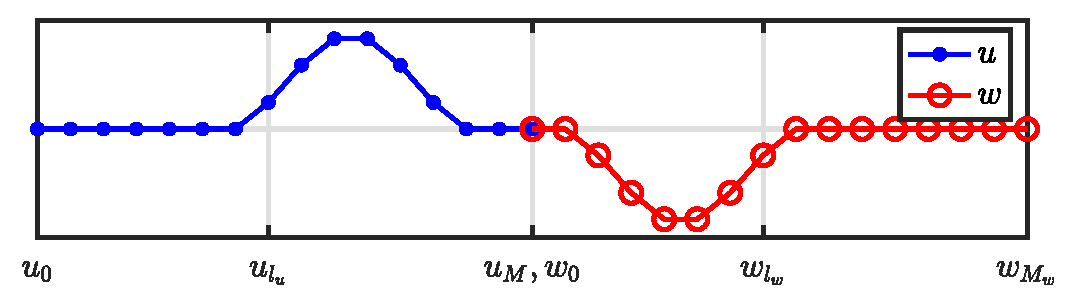
\includegraphics[width=\figwidth\columnwidth]{Figures/twoFreeStringsNarrow.eps}}}\\
    \vspace{-1em}\subfloat[]{\label{fig:twoFreeStringsGridMove}{ \includegraphics[width=\figwidth\columnwidth]{Figures/twoFreeStringsGridMoveNarrow.eps}}}\\
    \vspace{-1em}\subfloat[]{\label{fig:twoFreeStringsGridZoomed}{ \includegraphics[width=\figwidth\columnwidth]{Figures/twoFreeStringGridMoveZoomedNarrow.eps}}}
    \vspace{-1em}\caption{\it Illustration of the proposed method. In all figures, the x-axis shows the location of the respective grid points%(fx. $x_{u_l^n}$)
    , but `$x^n$' is omitted for brevity. (a) Locations of the states of two (1D wave) systems connected at the inner boundaries ($\Nfrac^n = 30$, $x_{u_{M^n}}^n = x_{w_0}^n$). (b) When $c^n$ -- and consequently $h^n$ -- are decreased and the positions of the grid points change ($\Nfrac^n = 30.5$, $x_{u_{M^n}}^n \neq x_{w_0}^n$). (c) Figure \ref{fig:twoFreeStringsGridMove} zoomed-in around the inner boundaries. The virtual grid points $u_{M^n+1}^n$ and $w_{-1}^n$ are shown together with the distance between them expressed using $\alpha$ in Eq. \eqref{eq:alphaDef}.}
\end{figure}

\subsubsection{Changing the Grid}\label{sec:changingGrid}
The previous section describes the case in which $\Nfrac^n$ is an integer. % $x_{u_M}^n = x_{w_0}^n$. 
We now continue by varying $c^n$ such that this is not the case.

The locations of the outer boundaries $x_{u_0}^n$ and $x_{w_{M_w}}^n$ are fixed:
\begin{equation*}
    x_{u_0}^n = x_{u_0}^0 = 0 \quad \text{and}\quad x_{w_{M_w^n}}^n = x_{w_{M_w^n}}^0 = L \quad \forall n.
\end{equation*}
If the wave speed $c^n$ is then decreased, and consequently the grid spacing $h^n$ according to Eq. \eqref{eq:stabilityCond} (with equality), all other points move towards their respective outer boundary (see Figure \ref{fig:twoFreeStringsGridMove}). Calculating $h^n$ this way allows this method to always satisfy the CFL condition in Eq. \eqref{eq:CFL} with equality, solving issues regarding simulation quality and numerical dispersion described in Section \ref{sec:quality}. %, as is the case with the previous iteration described in \ref{sec:iterations}.

% \begin{figure}[h]
% \centerline{\includegraphics[width=\columnwidth]{twoFreeStringGridMove} }
% \caption{\label{fig:twoFreeStringsGridMove}{When the grid changes ($\Nfrac = 30.5$). The x-axis shows the location (in m) of the respective grid points (fx. $x_{u_l^n}$), but the $x$ is omitted for clarity.}}
% \end{figure}

As mentioned in Section \ref{sec:systSetup}, the state of the virtual grid points at the inner boundaries are defined as $u_{M^n+1}^n = w_1^n$ and $w_{-1}^n = u_{M^n-1}^n$ when the inner boundaries perfectly overlap  (i.e., $x^n_{u_{M^n}} = x^n_{w_0}$). If this is not the case ($x^n_{u_{M^n}} \neq x^n_{w_0}$) a Lagrangian interpolator $I(x_i^n)$ at location $x_i^n$ (in m from the left boundary) can be used to calculate the value of these virtual grid points (also see Figure \ref{fig:twoFreeStringsGridZoomed} for reference). The interpolator $I$ is a row-vector with the same length as $\mathbfcal{U}^n$ (from Eq. \eqref{eq:fullState}) and its values depend on the interpolation order. %Furthermore, the rigid connection in \eqref{eq:rigid} is only valid when the inner boundaries perfectly overlap and does not have to be satisfied when $x_{u_M}^n \neq x_{w_0}^n$. 
In the following, the fractional part of $\Nfrac^n$ %distance between the inner boundaries normalised by $h$ 
is defined as 
\begin{equation}\label{eq:alphaDef}
    \alpha = \alpha^n = \Nfrac^n - N^n %\frac{x^n_{w_0} - x^n_{u_M}}{h}\,,
\end{equation}
and for clarity, $I$ and $\mathbfcal{U}^n$ are indexed by $m$.
%\SWcomment[it's possible to skip until quadratic interpolation straight away from here, skipping the iterations] In the following, the distance between the inner boundaries normalised with $h$ is defined as
% \begin{equation}\label{eq:alphaDef}
%     \alpha = \alpha^n = \frac{x^n_{w_0} - x^n_{u_M}}{h}\,,
% \end{equation}
% and for clarity, $I$ and $\mathbfcal{U}^n$ are indexed by $m$.
% Applying the interpolator to $\mathbfcal{U}^n$ yields
% \begin{subequations}\label{eq:interpolationGeneral}
%     \begin{align}
%         u_{M+1}^n &= I^\flip(x^n_{u_{M+1}})\mathbfcal{U}^n% = (1-\alpha)w_1^n + \alpha w_0^n
%         \\
%         w_{-1}^n &= I(x^n_{w_{-1}})\mathbfcal{U}^n,% = (1-\alpha)u_{M-1}^n + \alpha u_M^n
%     \end{align}
% \end{subequations}
% where $I^\flip$ is a flipped and shifted version of $I$.
% % where
% % \begin{equation}
% %     \alpha = \frac{x_{w_0} - x_{u_M}}{h},
% % \end{equation}
% % and grid-point locations $x_{u_{M+1}}$ and $w_{-1}$. Note that when $h$ changes the connected points start to move away from each other.
% %
% If linear interpolation is used, 
% \begin{subequations}\label{eq:linearInterp}
% \begin{equation}
%     I_1(x_i) = 
%     \begin{cases}
%         (1-\alpha), & m = m_i \\
%         \alpha, & m = m_i + 1\\
%         0, & \text{otherwise}
%     \end{cases}
% \end{equation}
% and
% \begin{equation}\label{eq:linearFlip}
%     I_1^\flip(x_i) = 
%     \begin{cases}
%         \alpha, & m = m_i^\flip \\
%         (1-\alpha), & m = m_i^\flip + 1\\
%         0 & \text{otherwise}
%     \end{cases}
% \end{equation}
% \end{subequations}
% with $m_i = \lfloor x_i/h\rfloor$ and $m_i^\flip = \lfloor x_i/ h+(1-\alpha) \rfloor$, where the shift in the latter is necessary to transform the location $x_i$ to the right indices of $\mathbfcal{U}^n$. Substituting \eqref{eq:linearInterp} into \eqref{eq:interpolationGeneral} and expanding yields
% \begin{subequations}
%     \begin{align}
%         u_{M+1}^n &= I_1^\flip(x^n_{u_{M+1}})\mathbfcal{U}^n = \alpha w_0^n
%         + (1-\alpha)w_1^n,\\
%         w_{-1}^n &= I_1(x^n_{w_{-1}})\mathbfcal{U}^n = (1-\alpha)u_{M-1}^n + \alpha u_M^n.
%     \end{align}
% \end{subequations}
% % \begin{figure}[h]
% % \centerline{\includegraphics[width=\columnwidth]{twoFreeStringGridMoveZoomed} }
% % \caption{\label{fig:twoFreeStringsGridZoomed}{When the grid changes (zoomed). The states at the inner boundaries $u_M$ and $w_0$ are shown together with virtual grid points $u_{M+1}$ and $w_{-1}$.}}
% % \end{figure}
% %
% Using $I_1$, analysis of the output shows that the expected fundamental frequency $f_0$ is slightly higher when interpolation needs to happen than the one expected when using Eq. \eqref{eq:fundamentalFreq}. Furthermore, modes higher than $f_\text{s} / 4$ would follow an odd pattern up when decreasing the wave speed, opposite of what is expected. \SWcomment[$\leftarrow$ didn't know where (or whether) to include this.]
%
% One could extend the range of interpolation by one point to each side, using a cubic Lagrange interpolator instead. Although this would require $w_{-1}^n$ to calculate $u_{M+1}^n$ and vice versa, it is possible to solve this by treating the interpolation equations as a system of linear equations. Analysis of this method, though yielding a correct $f_0$ at all times, shows similar behaviour to the linear interpolation, with odd behaviour regarding modes higher than $f_\text{s}/4$.
%
% Much better behaviour is observed when points of both $u_l^n$ and $w_l^n$ are used to calculate the values of the virtual grid points. This means to also use $u_M^n$ to calculate $u_{M+1}^n$ and $w_0^n$ for $w_{-1}^n$. Now, the locations of the grid points used in the interpolation are not equidistant and a custom Lagrangian interpolator needs to be created. The lowest order interpolator that can be used here is the quadratic interpolator $I_2$
%
% The best behaviour is observed when $I$ is even-ordered (odd-ordered interpolation results in higher-frequency modes %crossing and
% increasing as $c^n$ decreases and vice-versa) \SBcomment[Could possibly remove this, as it raises a lot of questions...] \MDcomment[I agree ... if you make a comment like this you'd have to give some proof of it.] \SWcomment[Just what is between the parentheses or more..?]. Although higher orders yield slightly better behaviour this improvement is negligible and the lowest even-ordered, quadratic interpolation, already yields good results. The quadratic interpolator $I_2$ is defined as \MDcomment[I would probably just leave out the whole paragraph and just say: "consider the following quadratic interpolator" ]
Now, consider the following quadratic interpolator
\begin{subequations}\label{eq:quadInterp}
\begin{equation}\label{eq:quadNonFlip}
    I_2(x_i^n) =
    \begin{cases}
        -(\alpha-1)/(\alpha + 1), & m = m_i^n-1\\
        1, & m = m_i^n\\
        (\alpha-1)/(\alpha + 1), & m = m_i^n+1\\
        0, & \text{otherwise}
    \end{cases}
\end{equation}
and its flipped version
\begin{equation}\label{eq:quadFlip}
    I_2^\flip(x_i^n) = 
    \begin{cases}
        (\alpha-1)/(\alpha + 1), & m = (m_i^\flip)^n-1\\
        1, & m = (m_i^\flip)^n\\
        -(\alpha-1)/(\alpha + 1), & m = (m_i^\flip)^n+1\\
        0, & \text{otherwise}
    \end{cases}
\end{equation}
\end{subequations}
with $m_i^n = \lfloor x_i^n/h^n\rfloor$ and $(m_i^\flip)^n = \lfloor x_i^n/ h^n+(1-\alpha) \rfloor$, where the shift in the latter is necessary to transform the location $x_i^n$ to the correct indices of $\mathbfcal{U}^n$.
When applied to Eq. \eqref{eq:fullState} this yields the definitions for the virtual grid points
\begin{subequations}\label{eq:connectionInterpol}
\begin{align}
        &u_{M^n+1}^n = I_2^\flip(x^n_{u_{M^n+1}})\mathbfcal{U}^n = \frac{\alpha - 1}{\alpha + 1}u_{M^n}^n + w_0^n - \frac{\alpha - 1}{\alpha + 1}w_1^n,
    \label{eq:calcUMP1}\\
        &w_{-1}^n = I_2(x^n_{w_{-1}})\mathbfcal{U}^n
        =-\frac{\alpha - 1}{\alpha + 1}u_{M^n-1}^n + u_{M^n}^n+ \frac{\alpha - 1}{\alpha + 1}w_{0}^n.\label{eq:calcWM1}
\end{align}
\end{subequations}
% where
% \begin{equation}\small
% \begin{gathered}\label{eq:interpolationCoeffs}
%     \alpha_\text{I} = \frac{\alpha(\alpha - 1)(\alpha - 2)}{-6}, \quad \beta_\text{I} = \frac{(\alpha - 1)(\alpha + 1)(\alpha - 2)}{2},\\
%     \gamma_\text{I} = \frac{\alpha(\alpha + 1)(\alpha - 2)}{-2}, \quad \text{and} \quad\delta_\text{I} = \frac{\alpha(\alpha + 1)(\alpha - 1)}{6}\,.
% \end{gathered}
% \end{equation}
% Treating \eqref{eq:connectionInterpol} as a system of linear equations, the virtual grid points $u_{M+1}^n$ and $w_{-1}^n$ can be solved for using
% \begin{equation}\label{eq:linSystSolution}
%     \begin{bmatrix}
%     u_{M+1}^n \\
%     w_{-1}^n
%     \end{bmatrix}
%     =
%     \mathbfcal{A}\begin{bmatrix}
%     \alpha_\text{I} w_2^n+ \beta_\text{I}w_1^n + \gamma_\text{I}w_0^n \\
%     \alpha_\text{I} u_{M-2}^n + \beta_\text{I}u_{M-1}^n + \gamma_\text{I} u_{M}^n
%     \end{bmatrix},
% \end{equation}
% where
% \begin{equation}\label{eq:Amat}
%     \mathbfcal{A} = \begin{bmatrix}
%          1 & -\delta_\text{I} \\
%          -\delta_\text{I} & 1
%     \end{bmatrix}^{-1}.\nonumber
% \end{equation}
% where
% \begin{equation}\nonumber
%     \mathbfcal{A} = \begin{bmatrix}
%          1 & -\delta_\text{I} \\
%          -\delta_\text{I} & 1
%     \end{bmatrix},
% \end{equation}
% and
% \begin{equation}\nonumber
%     \mathbf{v} = \begin{bmatrix}
%     \alpha_\text{I} w_2^n+ \beta\text{I}w_1^n + \gamma\text{I}w_0^n \\
%     \alpha_\text{I} u_{M-2}^n + \beta\text{I}u_{M-1}^n + \gamma u_{M}^n
%     \end{bmatrix}.
% \end{equation}
These definitions for the virtual grid points at the inner boundaries will replace the Neumann condition in Eq. \eqref{eq:halfStringBoundaryCondNeumann}. %As will be shown in Section \ref{sec:results}, quadratic interpolation yields the expected fundamental frequency at all times. 
One can show that when $\Nfrac^n$ is an integer, and thus $\alpha = 0$, Eqs. \eqref{eq:calcUMP1} and \eqref{eq:calcWM1} can be substituted as $w_1^n$ and $u_{M^n-1}^n$ into Eqs. \eqref{eq:resultUM} and \eqref{eq:resultw0} respectively (as these acted as virtual grid points $u_{M^n+1}^n$ and $w_{-1}^n$). Then recalling Eq. \eqref{eq:rigid} it can be seen that the system reduces to \eqref{eq:resultOneConnectedPoint} and exhibits the same exact behaviour as the normal case. % also when interpolation needs to happen.

Now that the virtual grid points at the inner boundaries are not determined by the Neumann boundary condition in \eqref{eq:halfStringBoundaryCondNeumann}, but rather by the definitions in Eqs. \eqref{eq:connectionInterpol}, system \eqref{eq:systemHalfStrings} can simply be re-written to
\begin{equation}\label{eq:FDSwithMethod}
    \begin{cases}
        \delta_{tt}u_\lu^n = (c^n)^2\delta_{xx}u_\lu^n\\
        \delta_{tt}w_\lw^n = (c^n)^2\delta_{xx}w_\lw^n
    \end{cases}
\end{equation}
where the Dirichlet condition in \eqref{eq:halfStringBoundaryCondDirichlet} is (still) used for the outer boundaries and the Neumann condition at the inner boundaries in \eqref{eq:halfStringBoundaryCondNeumann} is replaced by the definitions in \eqref{eq:connectionInterpol}:
\begin{equation}
        \!\!u_{M^n+1}^n = I_2^\flip(x_{u_{M^n+1}}^n)\mathbfcal{U}^n \quad \text{and}\quad w_{-1}^n = I_2(x_{w_{-1}}^n)\mathbfcal{U}^n.
\end{equation}
% Rewriting system \eqref{eq:systemHalfStrings} to include the method yields 
% \begin{equation}\label{eq:FDSwithMethod}
%     \begin{cases}
%         \delta_{tt}u_\lu^n = (c^n)^2\delta_{xx}u_\lu^n + J_u(x_{u_M}^n)2(c^n)^2\delta_{x\cdot}u_M^n\\
%         \delta_{tt}w_\lw^n = (c^n)^2\delta_{xx}w_\lw^n - J_w(x_{w_0}^n)2(c^n)^2\delta_{x\cdot}w_0^n
%     \end{cases}
% \end{equation}
% where the definitions for the virtual grid points from the second term are defined by the Neumann boundary condition in Eq. \eqref{eq:discreteNeumann} and those from the last terms are found in Eqs. \eqref{eq:connectionInterpol}. \SWcomment[actually it might be better (and more clear) to say that the Neumann condition at the inner boundaries is removed (such that to calculate $u_M^n$ and $w_0^n$ we need $u_{M+1}^n$ and $w_{-1}^n$) and the then-necessary virtual grid points are defined by Eqs. \eqref{eq:connectionInterpol}. Eventually comes down to the same thing... What do you think?]

\subsubsection{Adding and Removing Grid Points}\label{sec:addRemove}
When $c^n$, and consequently $h^n$, are decreased and the inner boundary points surpass the virtual points (i.e. $x_{u_{M^n}}^n \leq x_{w_{-1}}^n$ and $x_{w_0}^n \geq x_{u_{M^n+1}}^n$), this means that $N^n >  N^{n-1}$. A point is then added to the right boundary of $u$ and the left boundary of $w$ (for both time indices $n$ and $n-1$) in an alternating fashion: 
\begin{equation}\label{eq:addingPoint}
        \begin{cases}\mathbf{u}^n = [(\mathbf{u}^n)^T, I_3\mathbf{v}^n]^T & \text{if $N^n $ is odd},\\
        \mathbf{w}^n = [I_3^\flip\mathbf{v}^n, (\mathbf{w}^n)^T]^T & \text{if $ N^n$ is even},
        \end{cases}
\end{equation}
where 
\begin{align*}
\mathbf{v}^n = [u_{M^n-1}^n, u_{M^n}^n, w_0^n, w_1^n]^T,% \quad\text{and}\\
%     \mathbf{v}_\star^n &= [w_1^n, w_0^n, u_M^n, u_{M-1}^n],
\end{align*}
and cubic Lagrangian interpolator
\begin{equation}\label{eq:customIp}
    I_3 = \begin{bmatrix} -\frac{\alpha(\alpha+1)}{(\alpha+2)(\alpha+3)} &\frac{2\alpha}{\alpha+2} &\frac{2}{\alpha+2} 
    &-\frac{2\alpha}{(\alpha+3)(\alpha+2)}
    \end{bmatrix},
\end{equation}
with $I_3^\flip$ being a flipped, not shifted (as $I_2^\flip$ in Eq. \eqref{eq:quadFlip}) version of \eqref{eq:customIp}.
%with
% \begin{equation*}
%     \alpha' = \frac{x_{w_0}^n - (x_{u_M}^n + h)}{h}\ .
% \end{equation*}
See Figure \ref{fig:addingPoint}.
% Note that this operation is done for both time indices $n$ and $n-1$.
%
\begin{figure}[t]
    \centering
%% \reprintcolumnwidth is the same in preprint and reprint for
%% ease of use for authors:
\includegraphics[width=\figwidth\columnwidth]{Figures/addingGridPointNarrow.eps}
\caption{\label{fig:addingPoint}{\it The moment when a point is added to $\mathbf{u}$ at location $x_{u_{M^n+1}}^n$ in Eq. \eqref{eq:addingPoint}. This figure shows an extreme case where this location is far from $x_{w_0}^n$, i.e., $\alpha \not\approx 0$ in Eq. \eqref{eq:customIp}.}}
\end{figure}
Notice that $\Nfrac^n$ is only going to be slightly bigger than an integer at the moment that a point is added and Eq. \eqref{eq:alphaDef} will return $\alpha \gtrsim 0$.
%\MDcomment[Okay, I don't quite get this ... why cannot $\alpha$ be close to 1 here? In fact, it will be close to 1 when a point is about to be created ... I don't understand how the rate of change of $c$ affects the value of $\alpha$] \SWcomment[Right when a point is supposed to be added, $N^n$ is going to be slightly bigger than an integer value. Just to clarify, $N^n$ is first retrieved and then used to calculate $\alpha$ in \eqref{eq:alphaDef}. In quick parameter variations $N^{n-1}$ might be fx. 0.99, and $N^{n}$ fx. 0.3. Then $\alpha \not\gtrsim 0$. The way that the rate of change of $c$ is linked to $\alpha$ is that there is only $1/f_\text{s}$ seconds difference between $n$ and $n-1$.]
% ,  $\alpha$ in Eq. \eqref{eq:customIp} is expected to be close to zero, %, i.e., $x_{u_M}^n + h \approx x_{w_0}^n$,
This means that that $I_3 \approx [0, 0, 1, 0]$ and the displacement of the newly added point is nearly fully based on the grid point at the inner boundary of the other system. %This makes sense by looking at Figure \ref{fig:twoFreeStringsGridZoomed}, as exactly when the boundary points $u_M^n$ and $w_0^n$ surpass the virtual points $w_{-1}^n$ and $u_{M+1}^n$, these are going to be close to overlapping.

Removing grid points happens when $c^n$, and consequently $h^n$, are increased and $x_{u_{M^n}}^n > x_{w_0}^n$ (or $ N^n <  N^{n-1}$). %Compared to adding grid points, removing these is slightly more straightforward as points 
Grid points are simply removed from $\mathbf{u}$ and $\mathbf{w}$ (again for both $n$ and $n-1$) in an alternating fashion according to
\begin{equation}\label{eq:removingPoint}
\begin{cases}
    \mathbf{u}^n = [u_0^n, u_1^n ..., u_{M^n-1}^n]^T & \text{if $N^n$ is even}, \\
     \mathbf{w}^n = [w_1^n, w_2^n ..., w_{M_w^n}^n]^T & \text{if $N^n$ is odd}.
    \end{cases}
\end{equation}
In Eqs. \eqref{eq:addingPoint} and \eqref{eq:removingPoint}, the even and odd conditions can be inverted. To keep the difference between $u$ and $w$ a maximum of one grid point, the ceiling and flooring operations when calculating $M^n$ and $M_w^n$ will need to be inverted as well.

Until now, only adding and removing points in the center of the original system has been considered. This location could be moved anywhere along the grid, the limit being one point from the boundary. In other words, both $u_\lu^n$ and $w_\lw^n$ need to have at least one point (excluding the grid points at the outer boundaries). Furthermore, one does not have to add and remove points from $\mathbf{u}$ and $\mathbf{w}$ in an alternating fashion as in \eqref{eq:addingPoint}, but can just add to and remove from, for example, $\mathbf{u}$ leaving $\mathbf{w}$ the same size throughout the simulation. In the extreme case where $M^n = N^n - 1$ and $M_w^n = 1$ (leaving $w_\lw^n$ with only one moving grid point, $w_0^n$) the method still works.

\subsubsection{Displacement correction}\label{sec:dispCorr}
A problem that arises when increasing $c^n$, is that it is possible that the displacements $u_{M^n}^n \not\approx w_0^n$ at the time when a grid point needs to be removed. As the grid locations $x_{u_{M^n}}^n \approx x_{w_0}^n$ at the time of removal, this violates the rigid connection in \eqref{eq:rigid} and causes audible artifacts. A method is proposed that decreases the relative displacement of the inner boundaries the closer their grid-locations are together, i.e., the closer $\alpha$ in \eqref{eq:alphaDef} is to 0. We thus extend system \eqref{eq:FDSwithMethod} with an artificial spring force as
\begin{equation}\label{eq:sysDispCorr}
\begin{cases}
    \delta_{tt}u_\lu^n = (c^n)^2\delta_{xx}u_\lu^n+ J_u(x_{u_{M^n}}^n)%\left(2(c^n)^2\delta_{x\cdot}u_M^n + F_\text{c}^n\right)
    F_\text{c}^n,\\
    \delta_{tt}w_\lw^n = (c^n)^2\delta_{xx}w_\lw^n - J_w(x_{w_0}^n)%\left(2(c^n)^2\delta_{x\cdot}w_0^n+F_\text{c}^n\right)
    F_\text{c}^n.
\end{cases}
\end{equation}
Using centred temporal averaging and difference operators
\begin{subequations}\label{eq:centredOperators}
\begin{align}\label{eq:centredAverage}
    \mu_{t\cdot}\ugen_l^n &= \frac{1}{2} \left(\ugen_l^{n+1} + \ugen_l^{n-1}\right),\\
    \delta_{t\cdot}\ugen_l^n &= \frac{1}{2k} \left(\ugen_l^{n+1} - \ugen_l^{n-1}\right),
\end{align}
\end{subequations}
the correction effect %(in m$^2/$s$^2$) 
is defined as %\SWcomment[something off with the units here. I think I took this from the scaled version and assumed that $J$ has units of m$^{-1}$ (due to $1/h$).] is modelled as a spring-like connection and is defined as
\begin{equation}\label{eq:dispCorrForce}
    F_\text{c}^n = \beta \left(\mu_{t\cdot}\eta^n +\sigma_0\delta_{t\cdot}\eta^n \right).
\end{equation}
%\MDcomment[It seems that $\omega_0$ is somewhat redundant here.] \SWcomment[Actually, I did that for the units to add up (didn't have it before, as it is only the ratio between $\omega_0^2$ and $\sigma_0$ that matters..). As I plan to take away the units (since it's an arbitrary connection) should I remove it you think?] \MDcomment[Also, why multiply $\sigma_0$ by $\beta$? ... not very clear.] \SWcomment[$\beta$ simply scales the entire correction effect. Apart from force, I don't want there to be much damping effect when $\alpha$ is not close to 0 either.] 
with the difference in displacement between the inner boundaries
\begin{equation}\label{eq:etaDispCorr}
    \eta^n \triangleq w_0^n - u_{M^n}^n,
\end{equation}
and damping coefficient $\sigma_0$% (in s$^{-1}$)
. Furthermore, $\beta$ scales the effect of the displacement correction and is defined as
\begin{equation}\label{eq:betaDef}
    \beta = \beta(\alpha) = \frac{1-\alpha}{\alpha + \varepsilon}\ ,
\end{equation}
%(in m) \SWcomment[for the units to make sense... I guess it includes the $1/\rho A$ (for a 1D wave modelling a string without stiffness) but as it is an artificial connection force, it might make more sense to exclude all units here..] 
where $\varepsilon \ll 1$ prevents a division by 0. Despite the operators in \eqref{eq:centredOperators} introducing states at $n+1$, it is possible to calculate the force explicitly (such as in \cite{bilbao2009} or \cite{bilbao2009Dafx}). Furthermore, it can be shown that even when $\varepsilon = 0$ this calculation is always defined. In that case, as $\alpha \rightarrow 0$, $\beta\rightarrow \infty$ 
%\MDcomment[I don't quite get this. Why do you need to divide by $\alpha$ in (35)?] \SWcomment[To get $\beta \rightarrow \infty$ as $\alpha \rightarrow 0$ :)] \MDcomment[Also how is $\varepsilon$ chosen?] \SWcomment[It is set to 0 in the implementation. Do you think I should exclude it and just elaborate on the fact that even when $\beta \rightarrow \infty$ the calculation is defined?] \MDcomment[And how is the connection rigid when $\alpha = 0$?  Shouldn't a rigid connection have $\beta \rightarrow \infty$ ] \SWcomment[but it does! As I say, when $\epsilon = 0$ and $\alpha = 0$, $\beta\rightarrow \infty$. $\beta$ is simply a function that goes ("asymptotically") from $0$ to $\infty$ as $\alpha$ goes from $1$ to $0$] 
which acts as a rigid connection such as Eq. \eqref{eq:rigid}. Essentially, the displacement correction attempts to have $\eta^n\rightarrow 0$ in Eq. \eqref{eq:etaDispCorr} as $\alpha \rightarrow 0$ to satisfy the rigid connection in Eq. \eqref{eq:rigid}.
Although the correction presented here is not based on some physical process, it can be justified by the fact that large differences in displacement between two spatially adjacent points is not physical.

Notice that when $c^n$ is decreased, the rigid connection will not be violated as $u_{M^n}^n \approx w_0^n$ when a point is added. This is due to the fact that $I_3\approx [0, 0, 1, 0]$ and either $u_{M^n}^n$ or $w_0^n$ is the newly added point which almost solely based on the other (for low-speed parameter variations).
% \MDcomment[I have the feeling that this whole subsection is not very clear ... reviewers might jump on this, because there is no real justification for this extra spring system in here, outside of the fact that you hear artifacts and try to make up for it by adding this in. ] \SWcomment[I tried to justify at the beginning of \ref{sec:dispCorr} that differences in displacements while $\alpha \gtrsim 0$ violate the rigid connection and that this is a way to smoothly go towards this when increasing $c^n$. But I can see that this might not be enough. What do you propose? :)] \MDcomment[I don't know, it just looks strange that you need to do this. In fact, it's strange that you need two grids! Why not just work with one grid, where you fit the right boundary so to take into account the fractional grid spacing? Having two grids connected at the centre just sounds like a bit of a mess ...] \SWcomment[AHH entire method gone hahaha. No, been there, done that, unfortunately (as far as I know...). You can't do the quadratic interpolation then as you have too few points and you'll get weird behaviour with linear interpolation (as you might remember: modal crossings, opposite moving modal frequencies above $0.25 f_\text{s}$). And even there you'll need to "guide" the displacement of the grid point you're about to remove to the boundary value (which is 0 for Dirichlet) when decreasing $N$ as they will still have some "moment" or "inertia" from the $\delta_{tt}u$ term. In other words, right before removing a grid point, it will still be moving if it had earlier in the simulation, consequently, the Dirichlet boundary term will be violated, similar to how the rigid connection is violated here.\\
% One moving point with the proposed method is as close to adding / removing at the boundary as you'll get (as I describe in Section \ref{sec:addRemove}) and with a large system, this is basically the same as doing it at the boundary ;) I hope this all makes sense..]
% \MDcomment[It's just really strange that you are saying that (17) is valid $\forall$ n, when in fact in Fig 1 the points are far apart ... and here in 4.1.4 you are in fact saying that these points are not going to be equal. What is the point of introducing (17) then if you are going to have them connected with a spring? It seems that (17) is never really implemented ...
% Also, what is the purpose of the loss in the spring?] \SWcomment[You're right about the $\forall n$ in \eqref{eq:rigid}, I changed that and added to the condition that the rigid connection only holds when the inner boundaries perfectly overlap ($\alpha = 0$). The damping is so that you don't get highly oscillatory behaviour when $\alpha \gtrsim 0$. At least, that is what I observed. The damping lets the grid points at the inner boundaries go closer and closer together (more and more satisfying the rigid connection).]
% \MDcomment[It just looks not very well justified. There is not real ground to make these claims ... something reviewers will certainly notice!] \SWcomment[I'll try to justify it a bit more. Thanks!]
%$\beta$ can be seen as a spring force pulling the inner boundaries to the average displacement between them. A lower $\varepsilon$ decreases the chance of artifacts but will have a greater filtering effect on the system. For low-speed changes, using $\sim 1000$ samples for removing one grid point, $\varepsilon \approx 30$ ensures that $u_M^n \approx w_0^n$ at the time of removal and already suffices to remove artifacts.

% 
% \SWcomment[The following applies to odd-ordered Lagrange interpolators $\rightarrow$] The location at where points are added and removed greatly influences the behaviour of the system, especially in the higher frequencies (see Section \ref{sec:results}). The best behaviour is obtained when the location is as close to a boundary as possible. 

\subsection{Summary}
Here, Section \ref{sec:proposedMethod} is summarised and describes the final version of the proposed method.

The proposed method subdivides a grid function $\ugen_l^n$ with $N$ intervals into two grid functions $u_\lu^n$ and $w_\lw^n$ with $M^n$ and $M_w^n$ intervals respectively for a total of $N^n+2$ grid points. Knowing that $\lambda=1 \ \forall n$, Eq. \eqref{eq:updateEq}, written for both grid functions, becomes 
\begin{subequations}\label{eq:uwUpdates}
    \begin{align}
        u_\lu^{n+1} &= u_{\lu+1}^n + u_{\lu-1}^n - u_\lu^{n-1},\label{eq:uUpdate}\\
        w_\lw^{n+1} &= w_{\lw+1}^n + w_{\lw-1}^n - w_\lw^{n-1}\label{eq:wUpdate}.
    \end{align}
\end{subequations}
%
Due to the Dirichlet boundary condition in \eqref{eq:halfStringBoundaryCondDirichlet} imposed at the outer boundaries of the system, $u_0^n$ and $w_{M_w}^n$ are $0$ at all times and do not have to be included in the calculation. The ranges of calculation for Eq. \eqref{eq:uUpdate} and \eqref{eq:wUpdate} then become $\lu \in \{1, \hdots, M^n\}$ and $\lw \in \{0, \hdots, M_w^n - 1\}$ respectively. 

The grid points at the inner boundaries are calculated by expanding \eqref{eq:FDSwithMethod} (ignoring the displacement correction for now)
\begin{subequations}\label{eq:innerboundariesExpanded}
    \begin{align}
        u_{M^n}^{n+1} &= u_{{M^n}+1}^n + u_{{M^n}-1}^n - u_{M^n}^{n-1},\\
        w_0^{n+1} &= w_{-1}^n + w_{1}^n - w_0^{n-1}.
    \end{align}
\end{subequations}
%
where virtual grid points $u_{{M^n}+1}^n$ and $w_{-1}^n$ can be calculated using Eq. \eqref{eq:connectionInterpol}.

Then, when $ N^n > N^{n-1}$ a point is added to $\mathbf{u}^n$ and $\mathbf{u}^{n-1}$ (or $\mathbf{w}^n$ and $\mathbf{w}^{n-1}$) using Eq. \eqref{eq:addingPoint}, and when $ N^n  < N^{n-1}$ a point is removed from the same vectors using Eq. \eqref{eq:removingPoint}. In order to prevent audible artifacts when increasing $c^n$ (and thus decreasing $\Nfrac^n$) due to a violation of the rigid connection in \eqref{eq:rigid}, a method in \eqref{eq:sysDispCorr} is proposed to ensure that the grid points at the inner boundaries have a similar displacement when one of them is removed. 

% \MDcomment[I think it would be a lot cleaner if you wrote down the form of $Dxx$ and therefore gave a FD equivalent of (1). For the same reason, it would be better to stick to $\bf q$ for notation. So, you could have $\delta_{tt} {\bf Q}^n = c^n {\bf D}_{xx}{\bf Q}^n$] \SWcomment[Hmm.. but $\mathbf{D}_{xx}$ does not work here due to all the additional stuff (interpolation, displacement correction) right?] \MDcomment[You can definitely define a Dxx operator that includes all that, depending on alpha, beta, etc] \SWcomment[Actually, now that I don't do the modal analysis stuff in detail anymore I can just remove the matrixforms here (will also save some space) $\rightarrow$]
% Finally, using $\mathbfcal{U}$ from Eq. \eqref{eq:fullState} the total system can be compactly written in matrix form as
% \begin{equation}\label{eq:totalSystem}
%     \mathbf{C}_+^n\mathbfcal{U}^{n+1} = 
%     \mathbf{B}^n
%     \mathbfcal{U}^n
%     + \mathbf{C}_-^n\mathbfcal{U}^{n-1}
% \end{equation}
% with $ N^n \times N^n$ matrices
% \begin{equation}\label{eq:bMat}
%     \mathbf{B}^n = 
%     % \begingroup % keep the change local
%     % \setlength\arraycolsep{2pt}
%     \begin{bmatrix}[cccc|cccc]
%         & \ddots  &\ddots & & & & 0 & \\
%           & 1 & 0 & 1 & & & & \\
%          & & 1 & \frac{\alpha - 1}{\alpha + 1} & 1  & -\frac{\alpha - 1}{\alpha + 1} & \\ \cline{2-7}
%          & & -\frac{\alpha - 1}{\alpha + 1} & 1  & \frac{\alpha - 1}{\alpha + 1}  & 1 & & \\
%             & & & &1 & 0 & 1  \\
%             & 0 & &  &  &\ddots & \ddots &
%       \end{bmatrix}
%     %    \endgroup
% \end{equation}
% containing the effect of the general method described in Section \ref{sec:changingGrid} and
% \begin{equation}\label{eq:CMat}
%     \mathbf{C}_\pm^n = \pm\left(\mathbf{I}^n - \frac{\beta k^2 (\omega_0^2\pm\sigma_0/k)}{2}\mathbf{J}^n\boldsymbol{\eta}^n\right)
% \end{equation}
% containing the effect of the displacement correction described in Section \ref{sec:dispCorr} where $\mathbf{I}$ is the $ N^n \times N^n$ identity matrix and 
% \begin{equation}
%     \mathbf{J}^n = [\mathbf{0}_{M^n-1}, 1/h^n, -1/h^n, \mathbf{0}_{M_w^n-1}]^T
% \end{equation}
% and 
% \begin{equation}
%     \boldsymbol{\eta}^n = [\mathbf{0}_{M^n-1}, -1, 1, \mathbf{0}_{M_w^n-1}]
% \end{equation}
% are vectors of length $N^n$ and $\boldsymbol{0}_i$ is a zero-vector of length $i$.
%
% \begin{equation}\small
%     \mathbf{B} = \begin{bmatrix}[ccccccc|cc]
%     & &\ddots &\ddots & \ddots  & & \mathbf{0} & & \\
%      & & &1 & 0 & 1 & & \mathbf{0} & \\
%      & & &  & 1 & 0 & 1 & & \\
%      & &\mathbf{0} &  & \mathbfcal{A}_{1, 2}\alpha_\text{I} &\mathbfcal{A}_{1, 2}\beta_\text{I} + 1 &\mathbfcal{A}_{1, 2}\gamma_\text{I} & \mathbfcal{A}_{1, 1}(\gamma_\text{I}-\alpha_\text{I})& \\ \cline{2-8}
%      & & \mathbf{0} & &\mathbfcal{A}_{2, 2}\alpha_\text{I} &\mathbfcal{A}_{2, 2}\beta_\text{I}&\mathbfcal{A}_{2, 2}\gamma_\text{I} & \mathbfcal{A}_{2,1}(\gamma_\text{I} - \alpha_\text{I}) & 
%     \end{bmatrix}
% \end{equation}
%
% Notice that as $\alpha$ approaches $1$, $\mathbf{B}$ reduces to a matrix with ones on the diagonals next to the main diagonal and zeros elsewhere, which translates directly to the normal case in Eq. \eqref{eq:updateEq} with $\Nfrac^n = M^n + M_w^n + 1$. 

\subsection{Implementation}
A MATLAB implementation of the proposed method and audio examples can be found online\footnote{\href{https://github.com/SilvinWillemsen/DAFx21DynamicGridFiles/}{https://github.com/SilvinWillemsen/DAFx21DynamicGridFiles/}} and Algorithm \ref{alg:calcOrder} shows the order of calculation of this implementation. Especially important to take into account, is to only retrieve a change in $c^n$ at time index $n$ once before all other calculations. This is to ensure that $u_\lu^n$ and $w_\lw^n$ are calculated with the same $\alpha$ and $\beta$ for all $\lu$ and $\lw$.
\begin{algorithm}[ht]
    \setstretch{1.1}
    \fbox{\parbox{0.8\linewidth}
    {
        \While{application is running}
        {
            \begin{minipage}[c]{0.9\linewidth}
                Retrieve new $c^n$\\
                Calc. $h^n$ (Eq. \eqref{eq:stabilityCond} with equality)\\
                Calc. $\Nfrac^n$ and $N^n$ (Eqs. \eqref{eq:fundamentalFreq} and \eqref{eq:orderOfCalcGrid}) \\
                Calc. $\alpha$ (Eq. \eqref{eq:alphaDef})\\
                \If{$ N^n \neq N^{n-1} $}
                {
                    Add or remove point (Eq. \eqref{eq:addingPoint} or \eqref{eq:removingPoint})\\
                    Update $M^n$ and $M_w^n$
                }
                % \If{$\lfloor N^n\rfloor > \lfloor N^{n-1} \rfloor$}
                % {
                %     Add point (Eq. \eqref{eq:addingPoint})\\
                %     Update $M$ and $M_w$
                % }
                % \ElseIf{$\lfloor N^n\rfloor < \lfloor N^{n-1} \rfloor$}
                % {
                %     Remove point (Eq. \eqref{eq:removingPoint})\\
                %     Update $M$ and $M_w$
                % }
                % Calc. $\beta$ (Eq. \eqref{eq:betaDef})\\
                % Update $\mathbf{B}$ and $\mathbf{C}_\pm$ (Eqs. \eqref{eq:bMat} and \eqref{eq:CMat})\\
                % Calc. scheme (Eq. \eqref{eq:totalSystem})\\
                Calc. virtual grid points (Eqs. \eqref{eq:connectionInterpol})\\                Calc. $u_\lu^{n+1}$ and $w_\lw^{n+1}$ (Eqs. \eqref{eq:uwUpdates} and \eqref{eq:innerboundariesExpanded})\\
                Calc. and apply displacement corr. (Eq. \eqref{eq:dispCorrForce})\\
                Retrieve output\\
                Update states ($\U^{n-1} = \U^n$, $\U^n = \U^{n+1}$)\\
                Update $N^{n-1}$ ($N^{n-1} = N^n$)\\
                Increment $n$
            \end{minipage} 
            % \begin{minipage}[c]{0.4\linewidth}
            % -\\
            % \vspace{2em}(Eq. \eqref{eq:addingPoint})\\
            
            % (Eq. \eqref{eq:removingPoint})\\

            % \end{minipage}
            }
        }
    }
    \vspace{0.12cm}
    \caption{\it Pseudocode showing the order of calculations.\label{alg:calcOrder}}
\end{algorithm}
\section{Analysis and Results}\label{sec:results}
% \subsection{Expected behaviour}
% This section shows the analysis of the system presented in the previous section and its behaviour.
%\SWcomment[I forgot to talk about the fact that when looking at the state of the system over time, a "perfect raised cosine" gets "out of shape" as it passes the inner boundaries when $\alpha$ is not close to 0 or 1. The interpolation thus does introduce some behaviour alike numerical dispersion and should maybe be touched upon here..  (although this might naturally result from the fact that the modes are not integer multiples of the fundamental...)]
% \subsection{Energy \SWcomment[Added this for your (SB, MD) review]}
% \SWcomment[I guess the most important thing I want to highlight using this section is the fact that in the static case, the energy can be shown to be constant, even when $\alpha \neq 0$. This means that the proposed method (without displacement correction) does not introduce losses! 
% My question to you: do you see a way (perhaps from the last terms in system \eqref{eq:FDSwithMethod} or the boundary terms in Eq. \eqref{eq:boundaryTerms}) to prove that the total energy of the system is static when $\alpha$ is static?]

% The energy of system \eqref{eq:FDSwithMethod} (which after expansion at the inner boundaries simply becomes \eqref{eq:innerboundariesExpanded}) can be retrieved using energetic analysis techniques \cite{bilbao2009} and a weighted inner product yielding
% \begin{equation}
%     \delta_{t+}\left(\mathfrak{h}_u + \mathfrak{h}_w\right) = \mathfrak{b}_u + \mathfrak{b}_w
% \end{equation}
% with 
% \begin{align}
% &\begin{aligned}
%     \mathfrak{h}_u =&\  \frac{1}{2}\sum_{\lu=0}^{M-1}h\Big((\delta_{t-}u_\lu^n)^2 + c^2 (\delta_{x+}u_\lu^n)(\delta_{x+}u_\lu^{n-1})\Big) \\
%     &+ \frac{\epsilon}{4}h(\delta_{t-}u_M^n)^2,
% \end{aligned}
% \\
% &\begin{aligned}
%     \mathfrak{h}_w=&\ \frac{1}{2}\sum_{\lw=1}^{M_w} h\Big((\delta_{t-}w_\lw^n)^2+c^2(\delta_{x-}w_\lw^n)(\delta_{x-}w_\lw^{n-1}) \Big)\\
%     &+ \frac{\epsilon}{4}h(\delta_{t-}w_0^n)^2,
%     \end{aligned}
% \end{align}
% and 
% \begin{equation}\label{eq:boundaryTerms}
%     \begin{aligned}
%     \mathfrak{b}_u &= c^2(\delta_{t\cdot}u_M^n)\left((\delta_{x-}u_M^n)+\frac{\epsilon}{2}h(\delta_{xx}u_M^n)\right) \quad \text{and}\\
%     \mathfrak{b}_w &= c^2(\delta_{t\cdot}w_0^n)\left(-(\delta_{x+}w_0^n)+\frac{\epsilon}{2}h(\delta_{xx}w_0^n)\right)
%     \end{aligned}
% \end{equation}
% with $\epsilon = \alpha + 1$. \SWcomment[When $\alpha = 0$, $u_M^n = w_0^n$ and the boundary terms vanish. When $\alpha \rightarrow 1$ the boundary terms reduce to 
% \begin{equation}
%     \mathfrak{b}_u+\mathfrak{b}_w = -\frac{c^2}{2}\delta_{t+}\big(h(\delta_{x+}u_M^n)(\delta_{x+}u_M^{n-1})\big),  
% \end{equation}
% which is essentially the potential energy between the inner boundaries. See Appendix B.4 (p. 17) in \url{https://www.overleaf.com/project/5eec78b95071c2000121fff4} for a derivation.]
% \subsection{Static}
\subsection{Modes}
% In order to determine whether the proposed method yields an output with the correct frequency content in the static case, a spectrum is taken of the system's output. The system with $N=15.5$ (so $\alpha = 0.5$ in \eqref{eq:bMat}) at a sample rate of $f_\text{s} = 44100$ Hz is compared to the same system with $f_\text{s} = 88200$ Hz resulting in $N=31$ ($\alpha = 0$) for the same $f_0$ according to Eq. \eqref{eq:fundamentalFreq}. See Figure \ref{fig:spectra}.

% \begin{figure}[ht]
%     \centering
% %% \reprintcolumnwidth is the same in preprint and reprint for
% %% ease of use for authors:
% \includegraphics[width=0.8\columnwidth]{Figures/spectraDoubleSampleRateQuadratic.eps}
% \caption{\label{fig:spectra}{A system with $N = 15.5$ at $f_\text{s} = 44100$} compared to a system with $N = 31$ at $f_\text{s} = 88200$. Both are supposed to have the same fundamental frequency $f_0$ according to Eq. \eqref{eq:fundamentalFreq}.}
% \end{figure} 

% As expected, the output of the system at integer $N = 31$ contains partials at perfect integer multiples of $f_0$ (Eq. \eqref{eq:fundamentalFreq}). When this is compared to the output of the system with $N = 15.5$, one can observe that the lower partials are nearly perfectly overlapping, whereas higher partials exhibit slight downwards deviations, exponentially increasing with frequency.

% % \subsection{Dynamic}
%For a more detailed look at the behaviour of the system when $c$ is changed dynamically, 
% Rewriting \eqref{eq:totalSystem} in one-step form \cite{bilbao2009}, 
% \begin{equation}\label{eq:oneStepForm}
%     \begin{bmatrix}
%         \U^{n+1}\\
%         \U^n
%     \end{bmatrix} = 
%     \underbrace{\begin{bmatrix}
%         \mathbf{C}_+^{-1}\mathbf{B} & \mathbf{C}_+^{-1}\mathbf{C}_-\\
%         \mathbf{I} & \mathbf{0}
%     \end{bmatrix}}_{\mathbf{Q}}
%     \begin{bmatrix}
%         \U^n\\
%         \U^{n-1}
%     \end{bmatrix}
% \end{equation}
% allows for a modal analysis to be performed. For static parameters, the complex frequency of the $p$'th mode can be retrieved as
% \begin{equation}\label{eq:modalAnalysis}
%     s_p = \frac{1}{k}\ln \left(\text{eig}_p(\mathbf{Q})\right),
% \end{equation}
% where the frequency (in Hz) and damping (in $s^{-1}$) of the $p$'th mode can be retrieved using $f_p = \mathfrak{I}(s_p)/2\pi$ and $\sigma_p = \mathfrak{R}(s_p)$
% % \begin{equation}
% %     f_p = \mathfrak{I}(s_p)/2\pi \quad \text{and} \quad \sigma_p = \mathfrak{R}(s_p)
% % \end{equation}
% respectively. Here, $\mathfrak{I}(\cdot)$ and $\mathfrak{R}(\cdot)$ denote the `imaginary' and `real part of'. These definitions still hold for slow variations of $c$. 
Writing system \eqref{eq:sysDispCorr} in matrix form, one can perform a modal analysis while changing $c^n$ to obtain the frequencies and damping coefficients for each mode over time. As a test case, the wave speed of a system running at $f_\text{s} = 44100$ Hz is linearly varied from $c^0 = 2940$ ($\Nfrac^0 = 15$) to $c^{n_\text{end}} = 2205$ ($\Nfrac^{n_\text{end}} = 20$) where $n_\text{end} = t_\text{dur} f_\text{s}$ is the simulation length in samples and $t_\text{dur} = 10$ s. Grid points are added and removed as close to the right boundary as possible, i.e., $M^n = N^n-1$ and $M_w^n = 1$ (similar behaviour can be observed if $M^n = 1$ and $M_w^n = N^n-1$).  %, changing $\mathbf{Q}$ and thus the modal frequencies over time. %The displacement correction presented in Section. \ref{sec:dispCorr} is not included in this analysis ($\varepsilon \gg 1$), but will be elaborated on in Section \ref{sec:dispCorrRes}. 
The result of the analysis is shown in Figure \ref{fig:modalAnalysis} where higher damping (induced by the displacement correction) is indicated using thinner and bluer lines. Figure \ref{fig:spectrogram} shows the resulting spectrogram, with the displacement correction deactivated, of the system excited with $u_1^0 = 1$ and the output retrieved at $u_1^n$, and Figure \ref{fig:spectrogramDamp} shows a system with the same excitation but the change in $c^n$ inverted ($\Nfrac^n=20\rightarrow 15$) and displacement correction activated.

\begin{figure}[t!]
    \centering
    \subfloat[]{\label{fig:modalAnalysis}{ \includegraphics[width=0.96\columnwidth]{Figures/modalAnalysisDampingNarrow2.eps}}}\\
    \vspace{-1em}\subfloat[]{\label{fig:spectrogram}{ 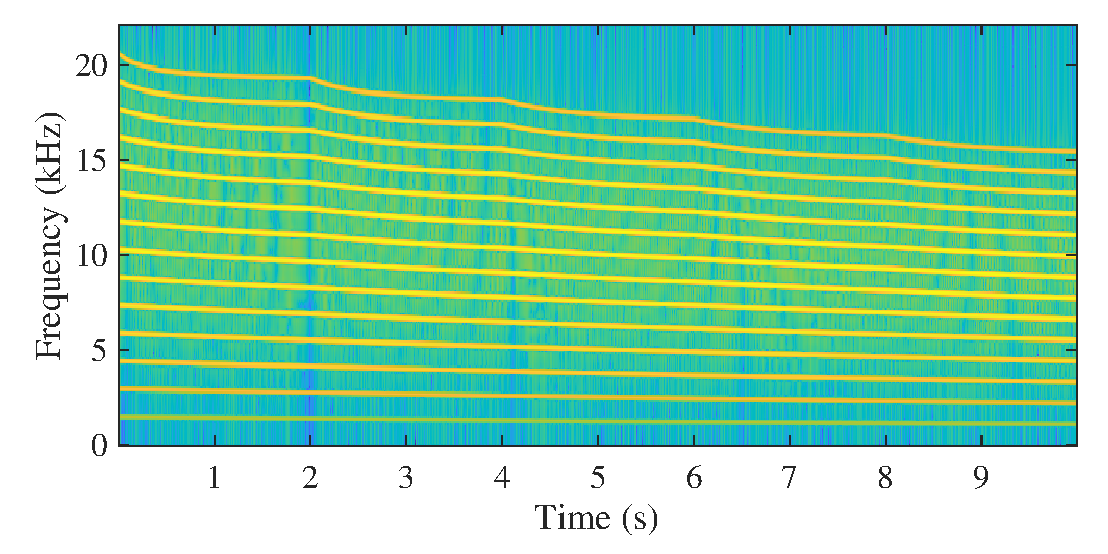
\includegraphics[width=0.95\columnwidth]{Figures/specQuadratic2NarrowNoScale.eps}}}\\
    \vspace{-1em}\subfloat[]{\label{fig:spectrogramDamp}{ 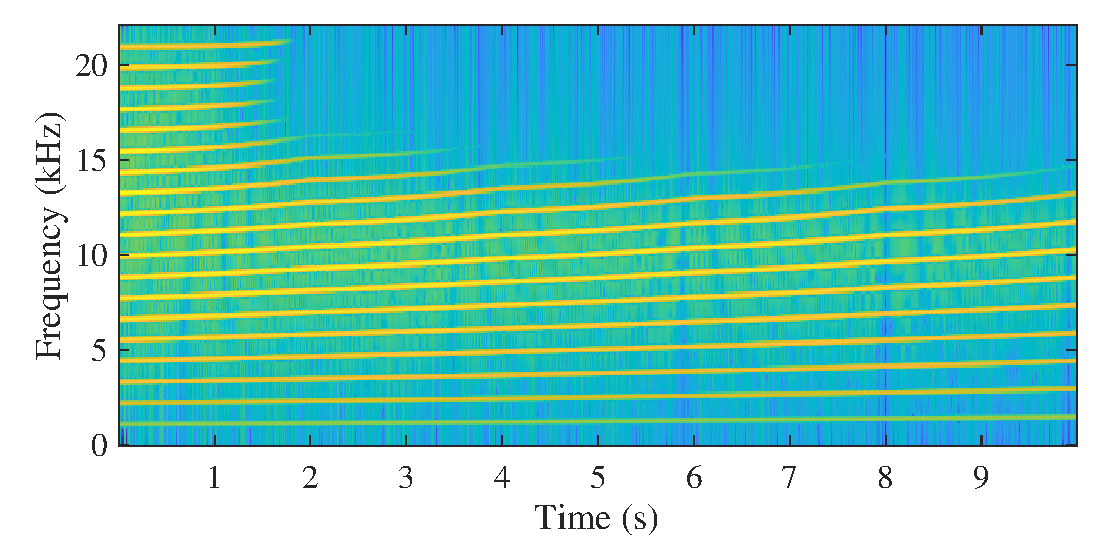
\includegraphics[width=0.95\columnwidth]{Figures/specQuadratic2DampNarrowNoScale.eps}}}
    \vspace{-1em}\caption{{\it Experiments showing (linearly) varying wave speed between $c^0 = 2940$ ($\Nfrac^0 = 15$) and} $c^{n_\text{end}} = 2205$ {\it (}$\Nfrac^{n_\text{end}} = 20$) {\it with $M^n = N^n - 1$ and $M_w^n = 1$ running at }$f_\text{s} = 44100$ {\it Hz for 10 s (}$n_\text{end} = 10f_\text{s}${\it ). (a) Modal analysis of system \eqref{eq:sysDispCorr}% using \eqref{eq:modalAnalysis}
    . Thinner and bluer lines indicate a higher amount of damping. (b) Output of the system while decreasing $c^n$ ($\Nfrac^n = 15 \rightarrow 20$) without displacement correction, excited using $u_1^0=1$ and retrieved at $u_1^n$. The sound output follows the same pattern as predicted by the analysis shown in Figure \ref{fig:modalAnalysis}. (c) Output of the system while increasing $c^n$ ($\Nfrac^n = 20 \rightarrow 15$) with displacement correction activated (essentially flipping the analysis in Figure \ref{fig:modalAnalysis} along the x-axis and applying this to a 10 s simulation).}\label{fig:analysisAndSpecs}}
\end{figure}
In the following, %\SWcomment[came up with this measure myself.. it made sense to me for measuring harmonic deviation / inharmonicity. Please let me know if you know a better measure or something I can reference]
% \begin{equation}
%     \varepsilon_p = \frac{f_p - pf_0}{f_0}\quad \text{[\%]}
% \end{equation}
% is used to calculate the harmonic deviation of mode $p$ from an integer multiple of the fundamental. Furthermore, 
the lowest mode generated by the analysis is referred to as $f_1^n$ and should ideally be equal to $f_0^n$ calculated using Eq. \eqref{eq:fundamentalFreqCont}. %To measure how much a mode deviates from a perfect harmonic, cents will be used \SWcomment[according to $1200\cdot\text{log}_2(f_p / pf_0)$].
%
The first thing one can observe from Figure \ref{fig:modalAnalysis} is that the frequencies of the modes decrease as $c^n$ decreases (as desired). The lower the mode, the more linear this decrease happens. Between $\Nfrac^n = 15$ and $\Nfrac^n = 16$, $f_1^n$ maximally deviates by $-0.15$ cents. In this same interval $f_{15}^n$ maximally deviates by $-67$ cents. This deviation %for mode number $p$
gets %progressively
less as $\Nfrac^n$ increases. %The maximum deviation for the highest mode number $f_{\lfloor N\rfloor}$, however, gets larger with a larger $N$, with $\text{max}(\varepsilon_{\lfloor N \rfloor})$ approaching $-100\%$ for extremely large values of $N$ ($>1000$). These deviations only happen between integer values of $N$ where at integer $N$ all modes are perfect integer multiples of $f_0$ and $\varepsilon_p = 0 \%$ for all $p$.
%
Experiments with higher even-ordered Lagrange interpolators show that these frequency deviations become smaller, but not by a substantial amount. The quadratic interpolator has thus been chosen for being simpler and more flexible while not being substantially worse than higher order interpolators.

Another observation from Figure \ref{fig:modalAnalysis} is that there are always $N^n$ modes present, corresponding to the number of moving points of the system. As can be seen in Figure \ref{fig:spectrogram} the highest mode is not excited. If the system is excited when $\Nfrac^n$ is not an integer, the highest mode will also be excited.
Comparing the implementation of the system using this method with integer $\Nfrac^n$ (without changing $c^n$) to a normal implementation of the 1D wave equation (shown in Section \ref{sec:FDTD}) with $N^n = \Nfrac^n$, identical outputs are observed, even though the latter has $N^n-1$ moving points.

% Using the quadratic interpolation from \eqref{eq:connectionInterpol}, or any other even-ordered Lagrange interpolator for that matter, the modal frequencies of the system do not change based on location. Experiments done with odd-ordered Lagrange interpolators showed that better behaviour is observed when points are added / removed closer to the boundaries. 

\subsection{Displacement Correction}\label{sec:dispCorrRes}
In the experiments, $\sigma_0 = 1$ in Eq. \eqref{eq:dispCorrForce}. The displacement correction has a low-pass-comb-filtering effect on the system, where the position and amount of damped regions directly relates to the position of where grid points are added and removed. The best behaviour, i.e., least affecting lower frequencies, is when grid points are added and removed as close to the boundary as possible, i.e., $M^n = N^n - 1$, and only has one damped region as shown in Figures \ref{fig:modalAnalysis} and \ref{fig:spectrogramDamp}.

% Experiments with different rates of change in $c^n$ showed that artifacts appeared when the highest mode is not attenuated as a grid point is removed. \SWcomment[$\leftarrow$ check this again!!]

% As mentioned in Section \ref{sec:dispCorr}, the displacement correction works with low-speed parameter changes and indeed removes artifacts when grid points are removed. Analysis of a static system with non-integer $N$ does, however, show that the correction has a low-pass comb-filtering effect on the system. The filtering is stronger for a lower values of $\epsilon$ and $\alpha$. The location and amount of the notches is determined by the location of the inner boundaries along the grid, i.e., where along the grid the displacement correction is applied. The amount of notches is equal to $\text{min}(M, M_w)$.
%Notches appear at ca. $m_\text{f}f_\text{s}/{2M_\text{min}}$ Hz and undamped frequencies right in between those, where notch number $m_\text{f} = [1, \hdots, M_\text{min}]$ and $M_\text{min} = \text{min}(M,M_w)$ is the minimum distance in points between the boundary and the location of adding and removing. 
% For a dynamic system, the notches move around the frequency spectrum and overall yield a low-passing effect.

\subsection{Limit on Rate of Change of $c$}
The current implementation of the proposed method can only add or remove a maximum one point per sample using Eqs. \eqref{eq:addingPoint} and \eqref{eq:removingPoint}. The rate of change of $f_0^n$ according to \eqref{eq:fundamentalFreq} is thus limited by $|\Nfrac^n - \Nfrac^{n-1}| \leq 1$. Though this is the maximum limitation on speed, a much lower limitation needs to be placed to keep the system well-behaved. The usual stability and energy analyses performed on FD schemes are not valid anymore in the time-varying case. Frozen coefficient analysis as in \cite{Strikwerda1989} could be applied here and hold for slowly varying coefficients, but is left for future work. 
% Notes:
% In the case that $\alpha = 0$ in Eq. \eqref{eq:totalSystem} (and thus $x_{u_M} = x_{w_0}$), one could go up to adding two points at a time by adding $u_{M+1}^n$ according to Eq. \eqref{eq:addingPoint} and adding an extra point $u_{M+2}^n$ using \eqref{eq:calcVirtualGridPoints} (in this case $u_{M+2}^n = w_0^n$). This would, however, not work if $\alpha \neq 0$, as a point added to $\mathbf{u}^n$ with $x_\text{i} < w_0$ needs interpolator \eqref{eq:customIp} and $\alpha'$ would be greater than $1$. As Eq. \eqref{eq:customIp} only works if $0\leq \alpha' \leq 1$, it is best to abide condition \eqref{eq:pointCondition} to be safe. 

% No speed limit if
% \begin{equation}
%     \text{floor}(N^n) = \text{floor}(N^{n-1})\Rightarrow M^n = M^{n-1},
% \end{equation}
% i.e., if no points are added or removed from the system. 
\section{Discussion}\label{sec:discussion}
To decide whether the proposed method works satisfactory, the results presented in the previous section are compared to the method requirements listed in Section \ref{sec:dynamicGrid} (denoted by r\# for short). 

It can be argued that the frequency deviations of $f_1^n$ from $f_0^n$ are sufficiently small to say that the r1 is satisfied. As for r2, a fractional number of intervals $\Nfrac^n$ has been introduced and smooth transitions are indeed observed from Figure \ref{fig:spectrogram}, in the case when $c^n$ is decreased and $\Nfrac^n$ is increased. When $c^n$ is increased instead, the displacement correction prevents artefacts when grid points are removed as seen in Figure \ref{fig:spectrogramDamp}. However, the filtering effect that the displacement correction has on the system (mentioned in Section \ref{sec:dispCorrRes}) is not ideal as it creates notches in the spectrum of the output sound. The least intrusive filtering happens when points are added and removed as close to the boundary as possible, i.e., when $M^n = 1$ or $M_w^n = 1$ where the notch only occurs in the higher end of the spectrum. As mentioned, artefacts are already removed when the highest mode is attenuated when a grid point is removed, so the current choice for $\omega_0$ and $\sigma_0$ in Eq. \eqref{eq:dispCorrForce} might be too high. As the displacement correction acts as a filtering operation, higher speeds of parameter variation will possibly cause the highest mode to not be filtered out `in time'. The values of $\omega_0$ and $\sigma_0$ could therefore also by made dynamic and depending on the rate of change of $c^n$ to have a higher effect when $c^n$ is increased faster and vice versa.
Either way, as this is still not ideal, another method for reducing artefacts that less affects the frequency content of the system should be devised, if possible. 

The modal analysis in Figure \ref{fig:modalAnalysis} shows that the method generates $N^n$ rather than $N^n - 1$ modes as set by r3. However, the output does contain the correct number of modes as shown in Figure \ref{fig:spectrogram} due to the highest mode not being excited. This is a result of the rigid connection imposed on the inner boundaries, forcing them to have the same displacement and act as one point. As mentioned in the results, when the system is excited at a non-integer $\Nfrac^n$, the highest mode is excited due to the fact that the inner boundaries can have different displacements in that case, but this is not an issue.
%
The latter part of r3, however, is not satisfied. The modes deviate from integer multiples of $f_0^n$, moreso for higher modes. Other interpolation techniques could be investigated to improve the behaviour and decrease this deviation.

Finally, the method only adds a few extra calculations for the inner boundaries so r4 is also easily satisfied. 
\\
% The fact that identical behaviour is observed at integer $N$ proves that at integer $N$ the method indeed reduces to the normal case confirming Section \ref{sec:systSetup}. If the system is excited when $N$ is not an integer, the highest mode will also be excited.

Although the results bring forward some drawbacks of the proposed method, such as modal frequency deviations, and filtering effects, most of these affect the higher frequencies of the output. First of all, human frequency sensitivity becomes very limited above 3000 Hz \cite{Zwicker1990} making high-frequency deviations much less important perceptually. Secondly, the physical systems one usually tries to model contain high-frequency losses, causing higher modes to usually not have very high amplitudes to begin with. Finally, $\Nfrac^n$ is usually much bigger in the systems that one tries to model, with which frequency deviations happen to a much smaller degree. 

% the analysis has been done on an extreme case: a lossless system with a small number of points. The issues presented, such as frequency deviations happen in higher frequencies. Physical processes usually lose the highest frequencies first so modes with higher frequencies usually do not have high amplitudes. This makes the frequency deviations of higher frequencies and the low-passing effect of the displacement correction much less apparent. 

\section{Conclusions and Perspectives}\label{sec:conclusion}
This paper presents a method to change grid configurations of finite-difference schemes to allow for dynamic parameter changes. The method allows the stability condition that these schemes rely on can be satisfied with equality at all times, minimising numerical dispersion and bandlimiting issues. Grid points are shown to be added and removed smoothly and do not cause artefacts when switching between grid configurations. 

The proposed method might not provide an exact solution to the problem of time-varying systems, and not all choices are physically justified, but it does circumvent the need for upsampling and higher orders of computations necessary to approximate this solution with, for example, full-grid interpolation. %Even though interpolation needs to happen, the drawbacks of full-grid interpolation can be avoided by not `listening' to the location where points are added but rather closer to the boundary. If one wants to listen to the center, the location where points are added or removed can easily be changed.
%
% Furthermore, the method allows the stability condition, which the scheme needs to abide, to always be satisfied with equality. This allows for a simulation where the parameters can be changed dynamically without running into either stability or quality issues, at least at slow parameter changes.

% The 1D wave equation was used as a test case, but the method could be used for other systems as well. 

Although this method has only been applied to the 1D wave equation it could be applied to many other 1D systems. Other parameters, such as material density or stiffness could also be made dynamic, going beyond what is physically possible. An application of the method that could be investigated is that of non-linear systems, such as the Kirchhoff-Carrier string model \cite{Carrier1945} where the tension is modulated based on the state of the system.

Other future work includes creating an adaptive version of the displacement correction that changes its effect depending on the speed at which the grid is changed. Finally, stability and energy analyses will have to be performed to show the limits on changes in parameters and grid  configurations.


% \section{Acknowledgments}
% Many thanks to the great number of anonymous reviewers!

%\newpage
\nocite{*}
{\small
\bibliographystyle{IEEEbib}
\bibliography{DAFx20_tmpl} % requires file DAFx20_tmpl.bib
}

\end{document}
